%--------------------------------------------------------------------------
%	PACKAGES AND OTHER DOCUMENT CONFIGURATIONS
%--------------------------------------------------------------------------
\documentclass[12pt,a4paper]{article}
\usepackage[utf8]{inputenc}
\usepackage[francais]{babel}
\usepackage[T1]{fontenc}
\usepackage{amsmath}
\usepackage{amsfonts}
\usepackage{amssymb}
\usepackage{graphicx}
\usepackage{lmodern}
\usepackage[left=2cm,right=2cm,top=2.2cm,bottom=2.2cm]{geometry}

\usepackage{fancyhdr} % Required for custom headers
\usepackage{lastpage} % Required to determine the last page for the footer
\usepackage{extramarks} % Required for headers and footers
\usepackage[usenames,dvipsnames]{color} % Required for custom colors
\usepackage{graphicx} % Required to insert images
\usepackage{caption}
\usepackage{subcaption}
\usepackage{listings} % Required for insertion of code
\usepackage{courier} % Required for the courier font
\usepackage{verbatim}
\usepackage{multirow}
\usepackage{eurosym}
\usepackage[squaren,Gray]{SIunits}

% Margins
%\topmargin=-0.45in
%\textwidth=6.5in
%\textheight=9.8in
\headsep=0.25in

% Set up the header and footer
%\pagestyle{fancy}
%\rhead{\firstxmark} % Top right header
%\lfoot{\lastxmark} % Bottom left footer
%\cfoot{} % Bottom center footer
%\rfoot{Page\ \thepage\ /\ \protect\pageref{LastPage}} % Bottom right footer
%\renewcommand\headrulewidth{0.3pt} % Size of the header rule
%\renewcommand\footrulewidth{0.3pt} % Size of the footer rule

\setlength\parindent{0pt} % Removes all indentation from paragraphs

%--------------------------------------------------------------------------
%	CODE INCLUSION CONFIGURATION
%--------------------------------------------------------------------------

\definecolor{MyDarkGreen}{rgb}{0.0,0.4,0.0} % This is the color used for comments
\lstloadlanguages{C} % Load C syntax for listings, for a list of other languages supported see: ftp://ftp.tex.ac.uk/tex-archive/macros/latex/contrib/listings/listings.pdf

\begin{document}
	
%--------------------------------------------------------------------------
%	TITLE PAGE
%--------------------------------------------------------------------------
\begin{titlepage}
\newcommand{\HRule}{\rule{\linewidth}{0.5mm}} % Defines a new command for the horizontal lines, change thickness here
\centering % Center everything on the page
 
%	HEADING SECTIONS
\null
\vspace{1cm}
\textsc{\Large Université Catholique de Louvain}\\[1cm] % Name of your university/college
\textsc{\large LINGI1113 \\[0.3cm] Systèmes informatiques 2}\\[0.5cm] % Major heading such as course name
%\textsc{\large Minor Heading}\\[0.5cm] % Minor heading such as course title

%	TITLE SECTION

\HRule \\[0.4cm]
{ \LARGE \bfseries Projet 2~: PIC horloge\\[0.4cm] % Title of your document
\large \bfseries Rapport} \\[0.4cm]

\HRule \\[0.5cm]
 
\begin{figure}[!h]
	\begin{center}
	%2048 × 1364
		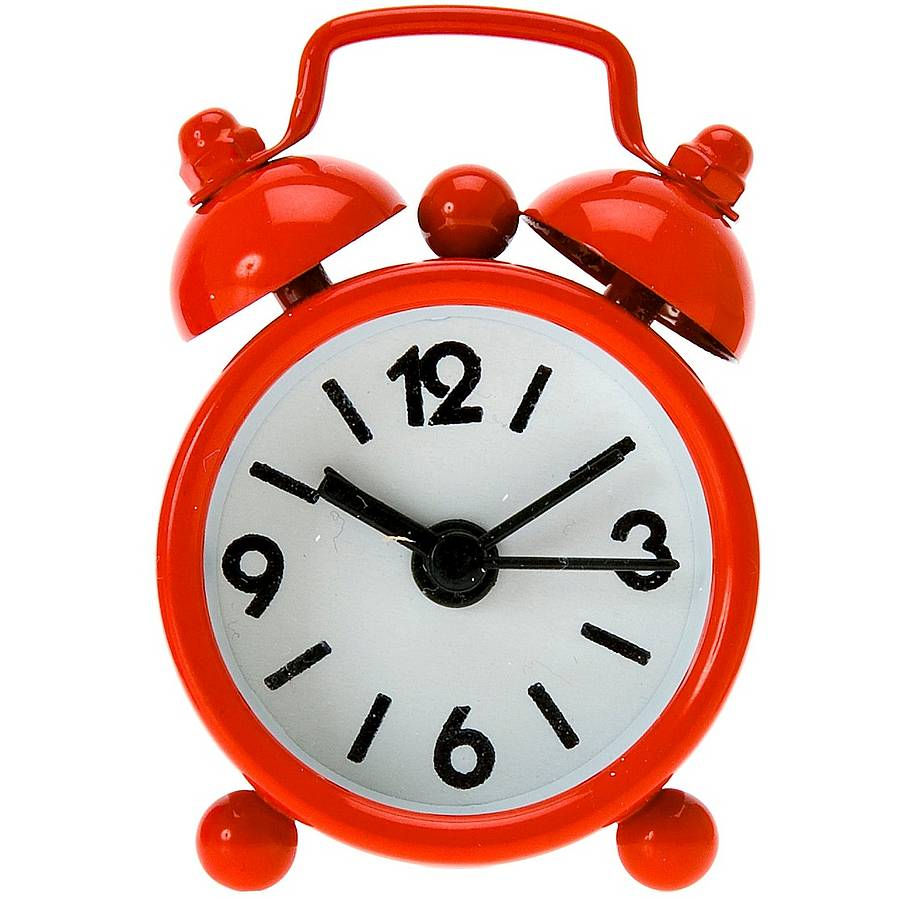
\includegraphics[width=10cm]{image.jpg}
	\end{center}
\end{figure}

%	AUTHOR SECTION

\large
\begin{centering}
Groupe 43\\
\end{centering}
{\begin{tabular}{lll}
\textsc{Peschke} & Lena & 5826 11 00\\
\textsc{Sedda} & Mélanie & 2246 11 00\\
\end{tabular}}
\\[1cm]

\normalsize
{\begin{tabular}{ll}
\textit{Professeur} : & Marc Lobelle \\
\end{tabular}}
\\[1cm]

%	DATE SECTION

{\normalsize \today} % Date, change the \today to a set date if you want to be precise

\newpage

\end{titlepage}

%--------------------------------------------------------------------------
%	TABLE OF CONTENTS
%--------------------------------------------------------------------------

\pagenumbering{gobble}
\clearpage
\thispagestyle{empty}
\tableofcontents
\clearpage
\pagenumbering{arabic}

%--------------------------------------------------------------------------
%	CONTENT
%--------------------------------------------------------------------------

\section{Introduction}

Le but de ce mini-projet a été de nous familiariser avec la programmation en C sur une machine dite ``nue'', c'est-à-dire sans réel système d'exploitation. Pour cela nous avons programmé un réveil matin sur une carte OLIMEX PIC MaxiWeb. Cette carte inclut un microcontrôleur de la firme Microchip et les programmes y ont un accès direct à la mémoire et aux périphériques. En particulier, nous avons dû utiliser nous-même les interruptions du ``timer'' pour déterminer l'heure.\\

Vous trouverez dans ce rapport des explications utiles pour l'utilisateur (c'est-à-dire tout ce qui concerne simplement l'utilisation du réveil lorsqu'il est déjà installé sur le PIC), pour l'installateur (les instructions décrivant comment compiler, installer sur le PIC et tester notre programme) et pour le programmeur (tout ce qui est nécessaire à un programmeur qui désirerait adapter notre programme). Dans cette dernière partie nous détaillerons notamment les spécifications de notre programme, la façon dont nous mesurons le temps qui passe, ainsi que nos divers choix d'implémentation.

\section{Documentation pour l'utilisateur}
% Le mode d'emploi de votre programme lorsqu'il est installé sur le PIC (documentation pour l'utilisateur)

Le réveil se compose de~:
\begin{itemize}
\item[1] écran LCD
\item[1] lampe LED jaune
\item[2] lampes LED rouges
\item[1] bouton MENU/NEXT/STOP (bouton 1, en bas)
\item[1] bouton SELECT/ADD/SNOOZE (bouton 2, en haut)
\end{itemize}

Il comporte un mode d'affichage, un menu de l'horloge et un menu de l'alarme.

\subsection{Réglages}

\begin{figure}[!h]
        \centering
        \begin{subfigure}[b]{0.5\textwidth}
                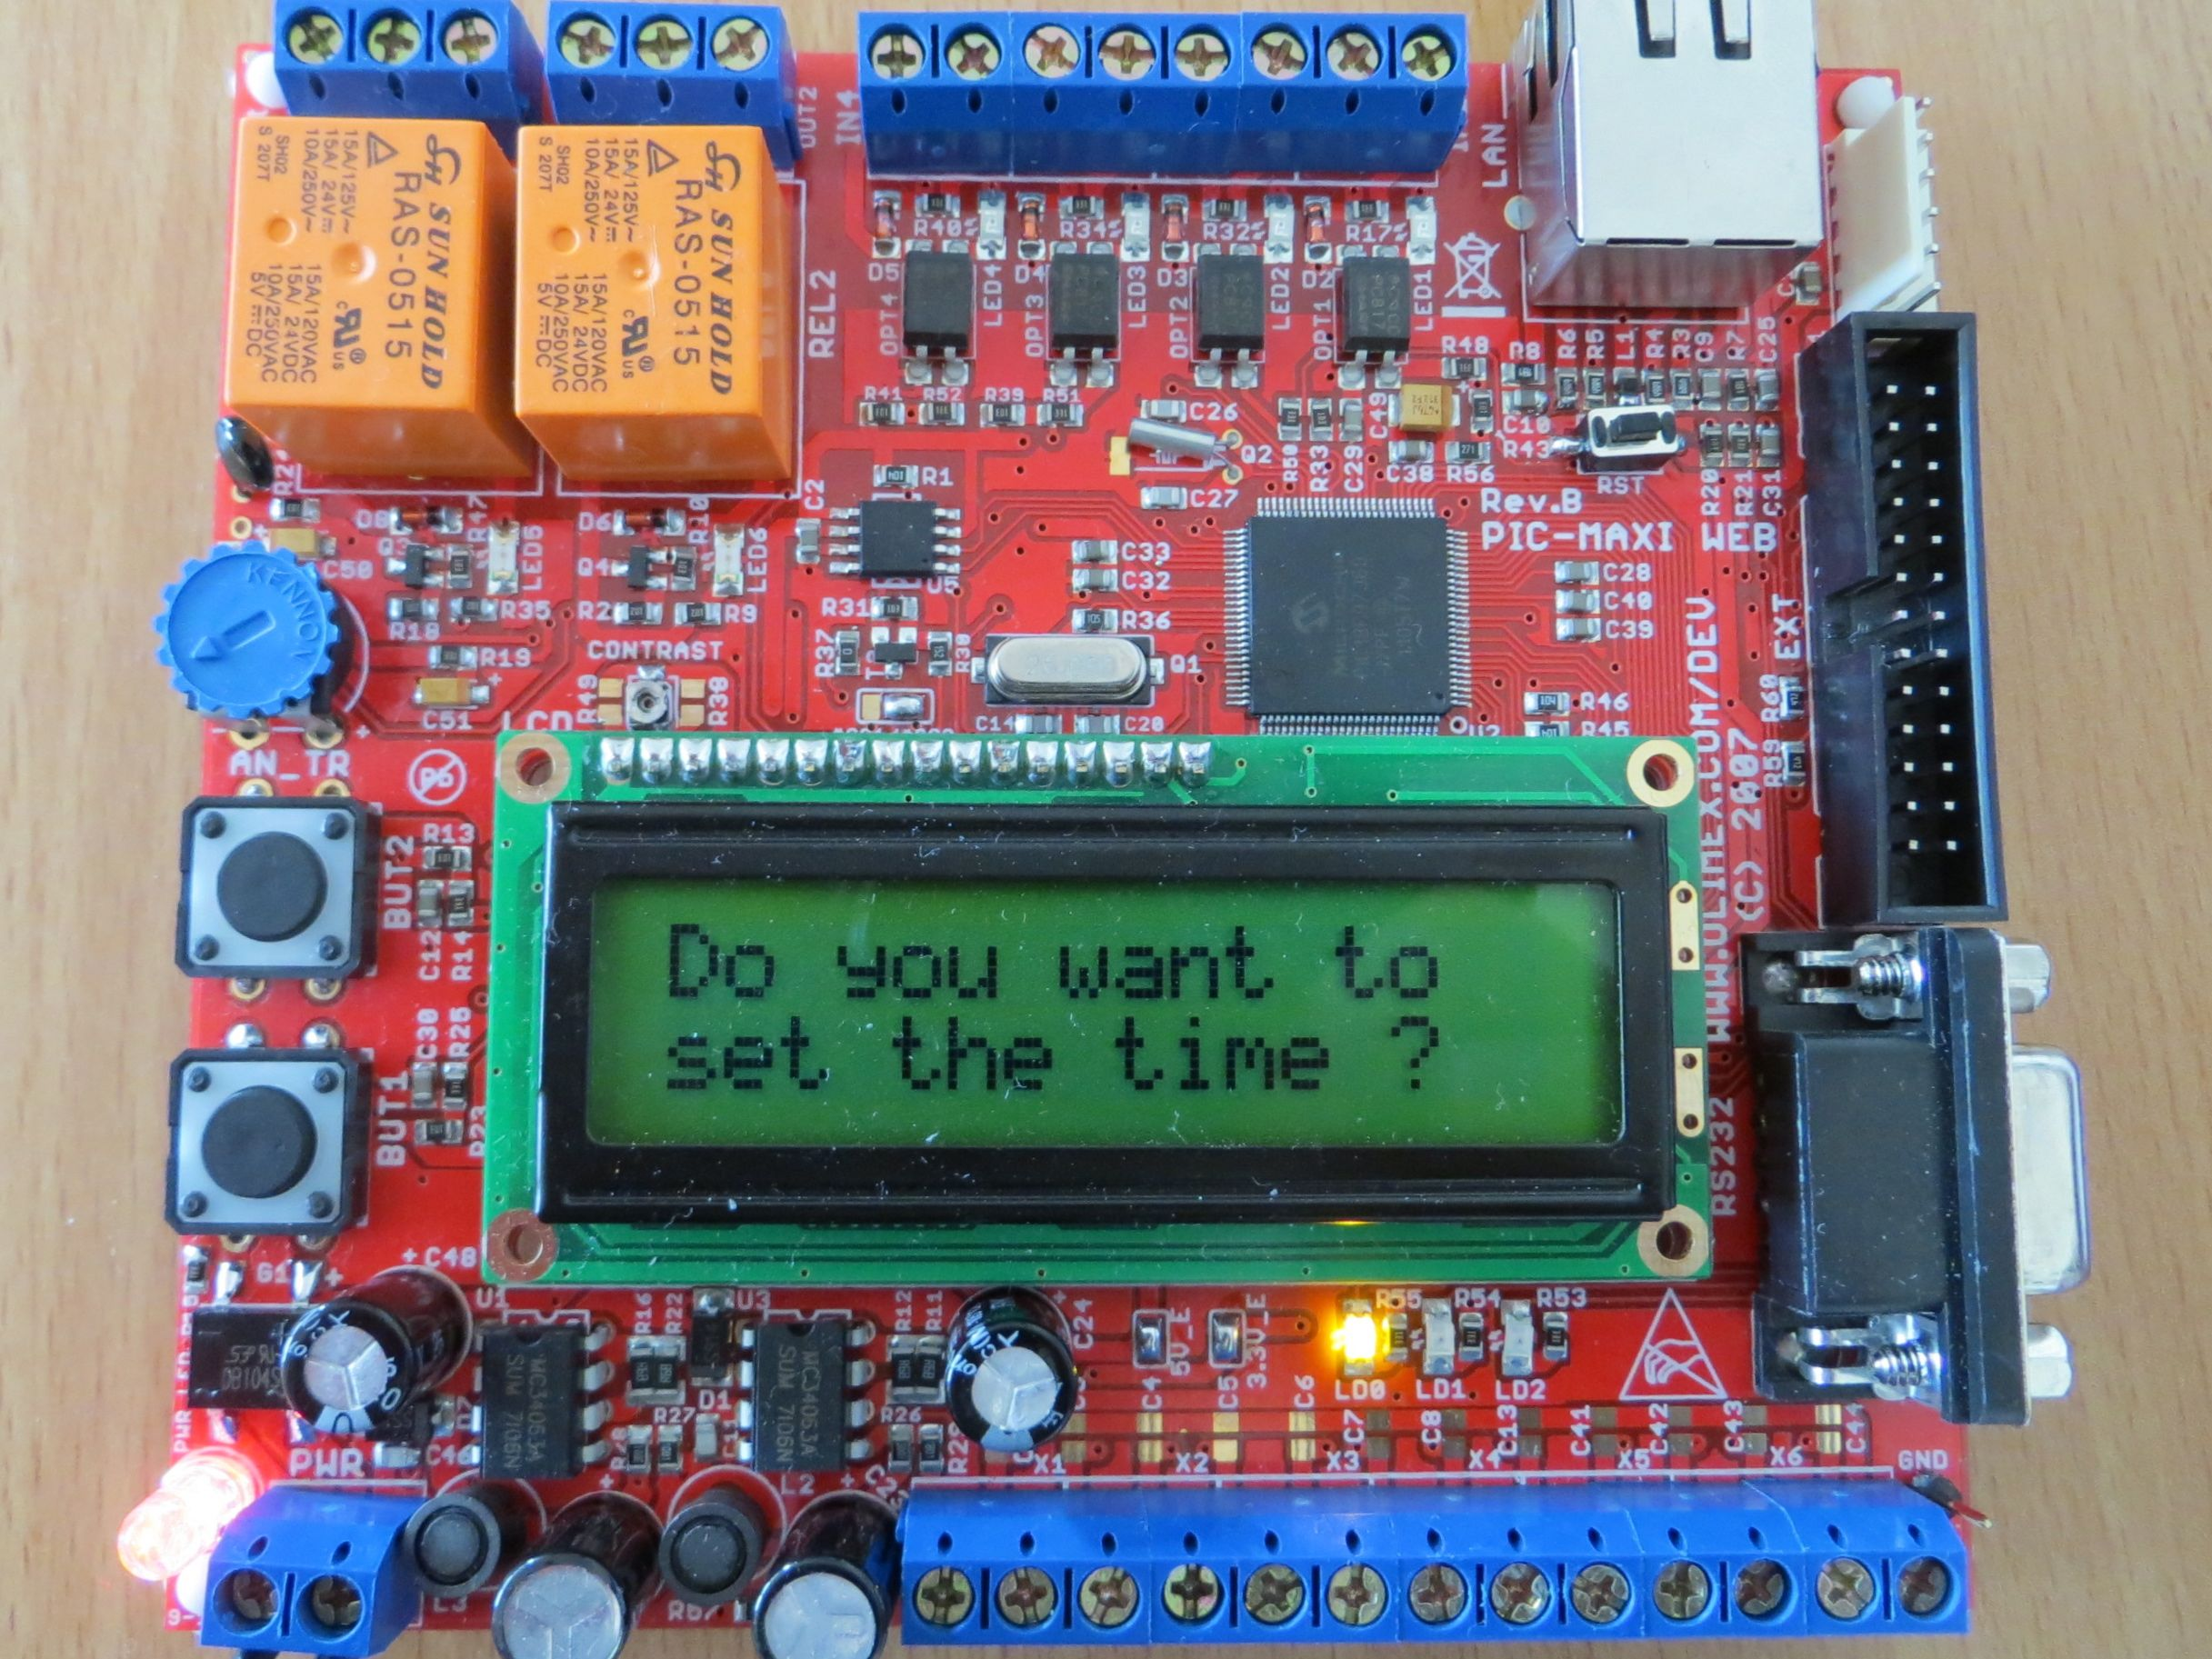
\includegraphics[width=\textwidth]{photos/IMG_2150.JPG}
                \caption{Menu}
                \label{fig:questionhorloge}
        \end{subfigure}%
        ~ %add desired spacing between images, e. g. ~, \quad, \qquad etc.
          %(or a blank line to force the subfigure onto a new line)
        \begin{subfigure}[b]{0.5\textwidth}
                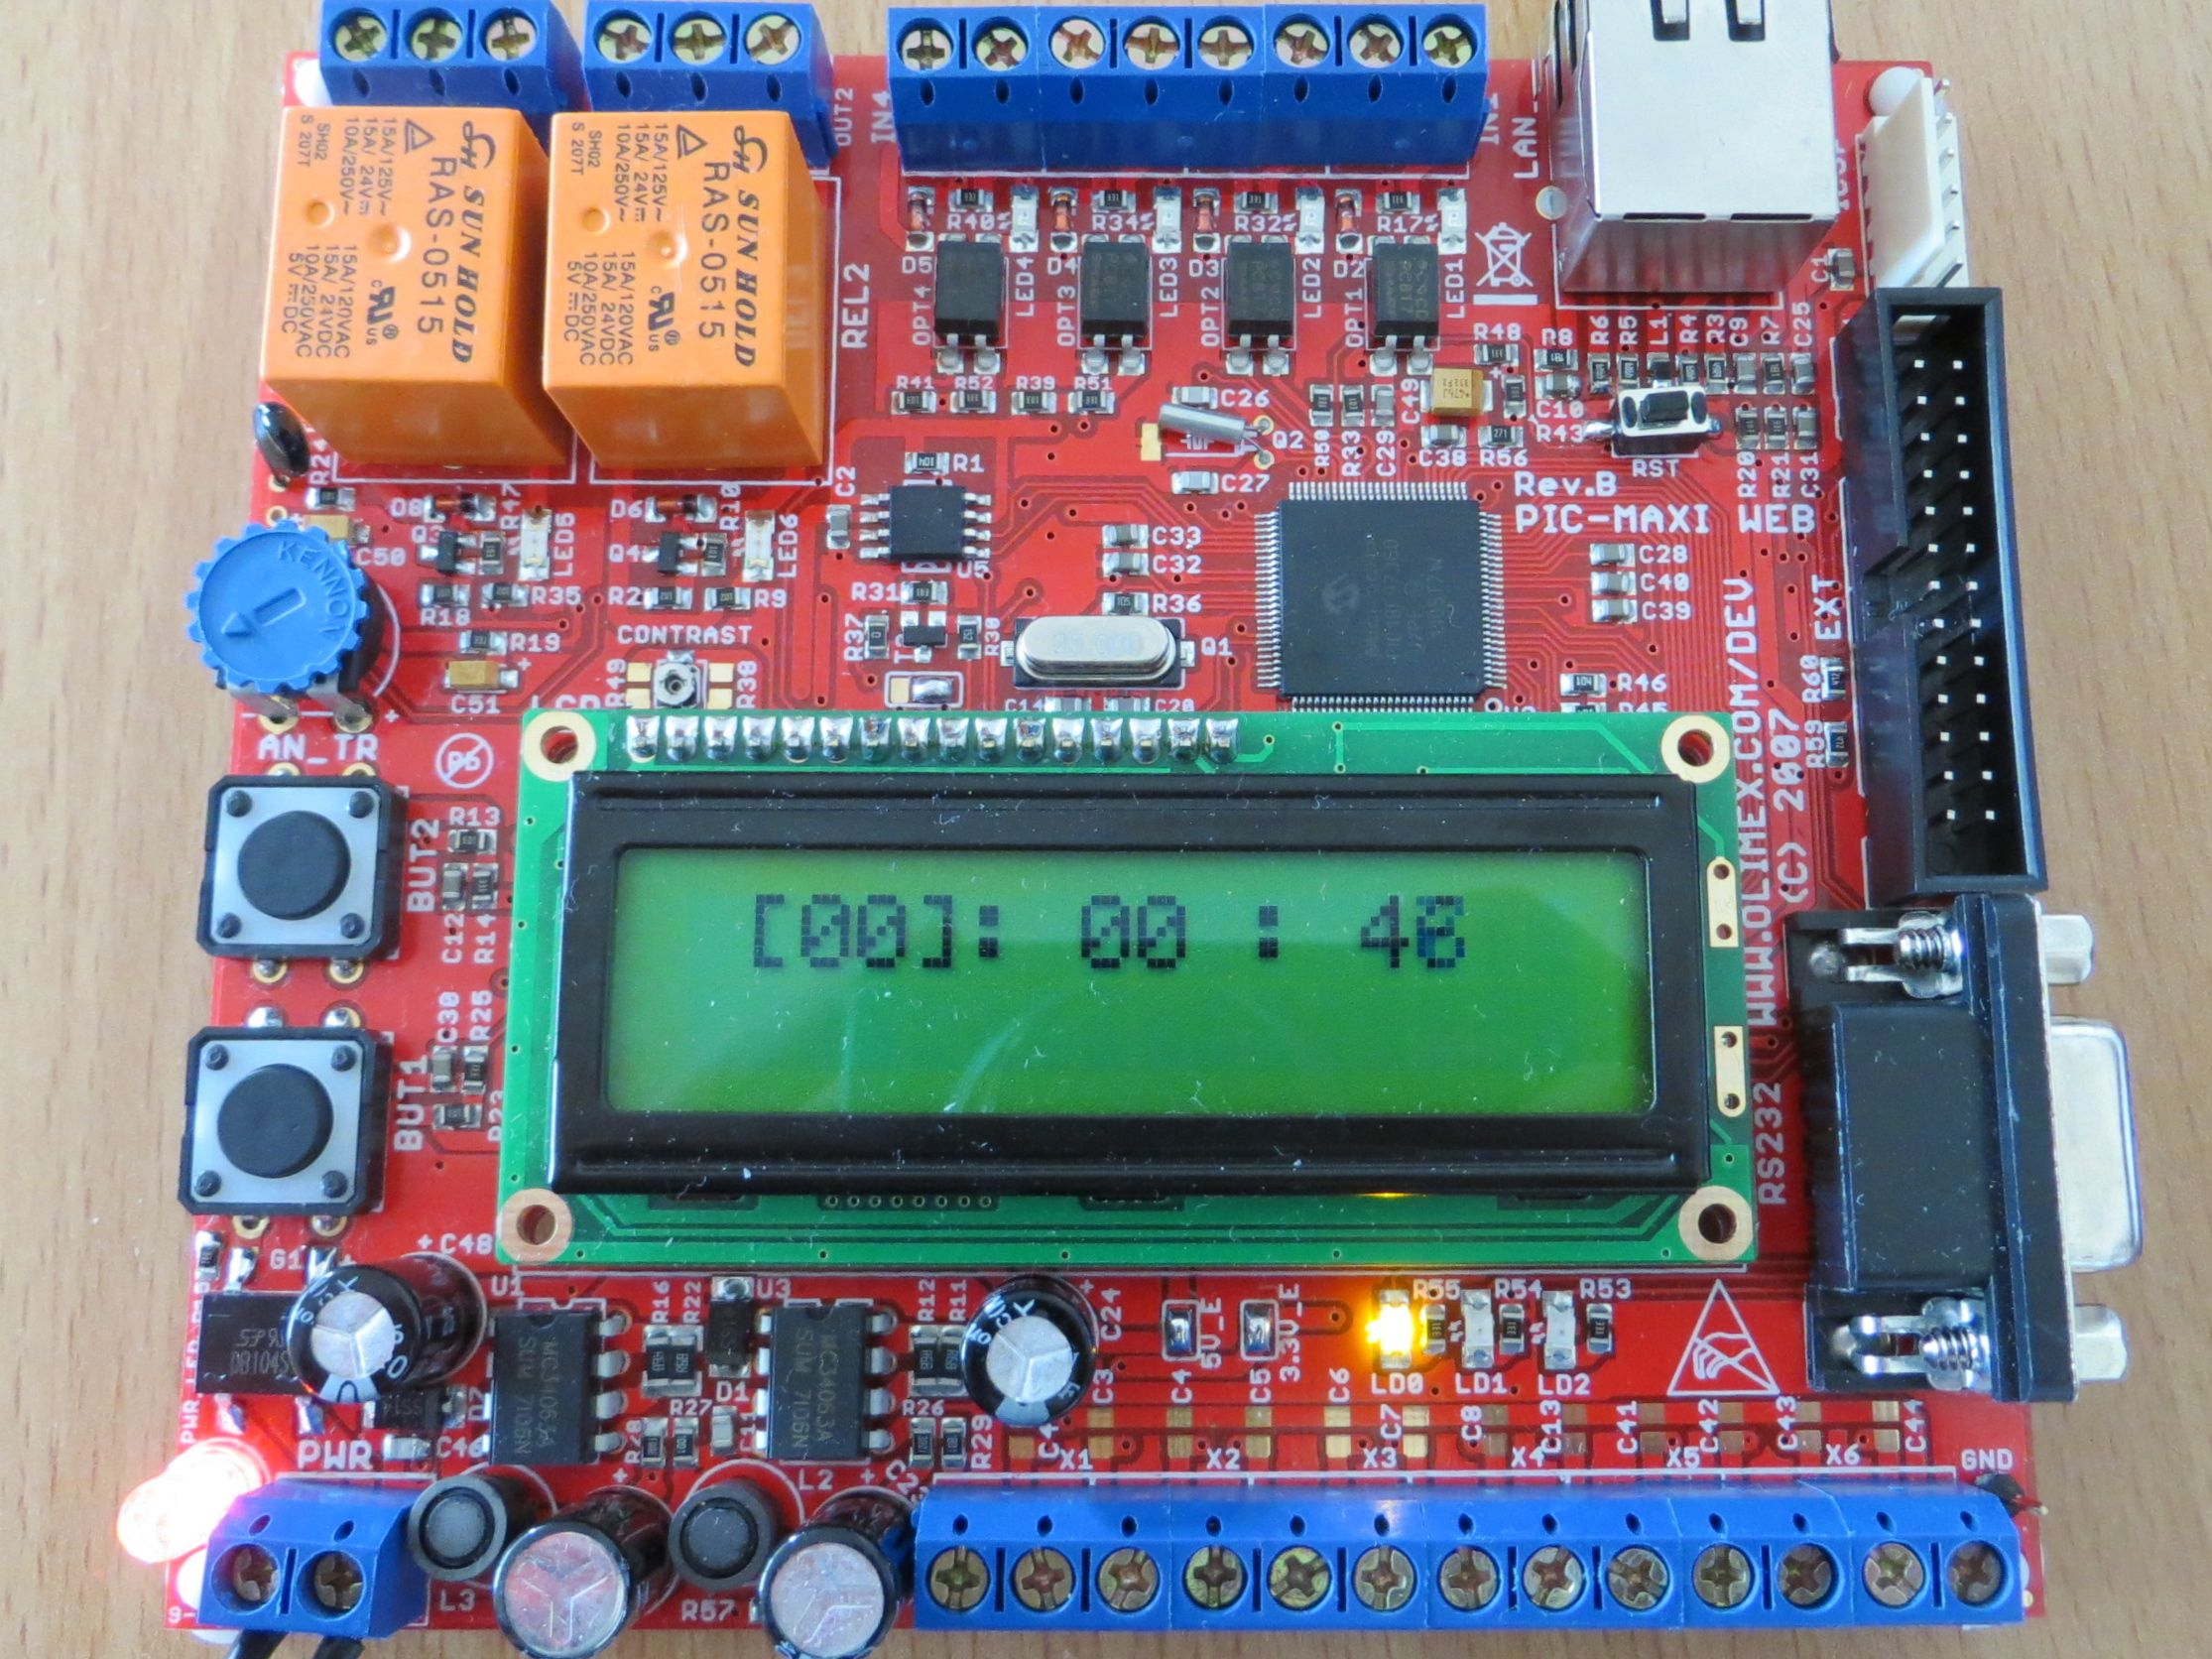
\includegraphics[width=\textwidth]{photos/IMG_2153.JPG}
                \caption{Modification de l'heure}
                \label{fig:modificationhorloge}
        \end{subfigure}
        \caption{Modification de l'heure de l'horloge}\label{fig:horloge}
\end{figure}

\paragraph{Première utilisation}
Par défaut, l'horloge commence à 00~:~00~:~00, l'alarme est désactivée et réglée pour 00~:~00. Nous proposerons uniquement à l'utilisateur de choisir l'heure et la minute du réveil parce que cela n'a pas beaucoup de sens de vouloir qu'il sonne à un nombre de secondes précis et c'est d'ailleurs ce qui se fait sur tous les réveils.  Lors de la mise sous tension du PIC, vous entrez dans le menu de l'horloge (Figure~\ref{fig:questionhorloge}).

\paragraph{Menu de l'horloge} L'accès au menu de l'horloge se fait via le bouton MENU. Une fois sur ce menu, vous pouvez soit appuyer sur le bouton NEXT pour passer au menu de l'alarme (Figure~\ref{fig:questionalarme}), soit poussez sur SELECT pour pouvoir changer l'heure (Figure~\ref{fig:modificationhorloge}).
Vous pouvez maintenant incrémenter les heures en appuyant sur ADD. Pour passer aux minutes et ensuite aux secondes, il suffit d'appuyer sur NEXT successivement, et de les augmenter en poussant ADD. Les crochets vous indiquent quelle valeur est en cours de modification.
Arrivé aux secondes, le bouton NEXT vous donne accès au menu de l'alarme (Figure~\ref{fig:questionalarme}).

\begin{figure}[!h]
        \centering
        \begin{subfigure}[b]{0.4\textwidth}
                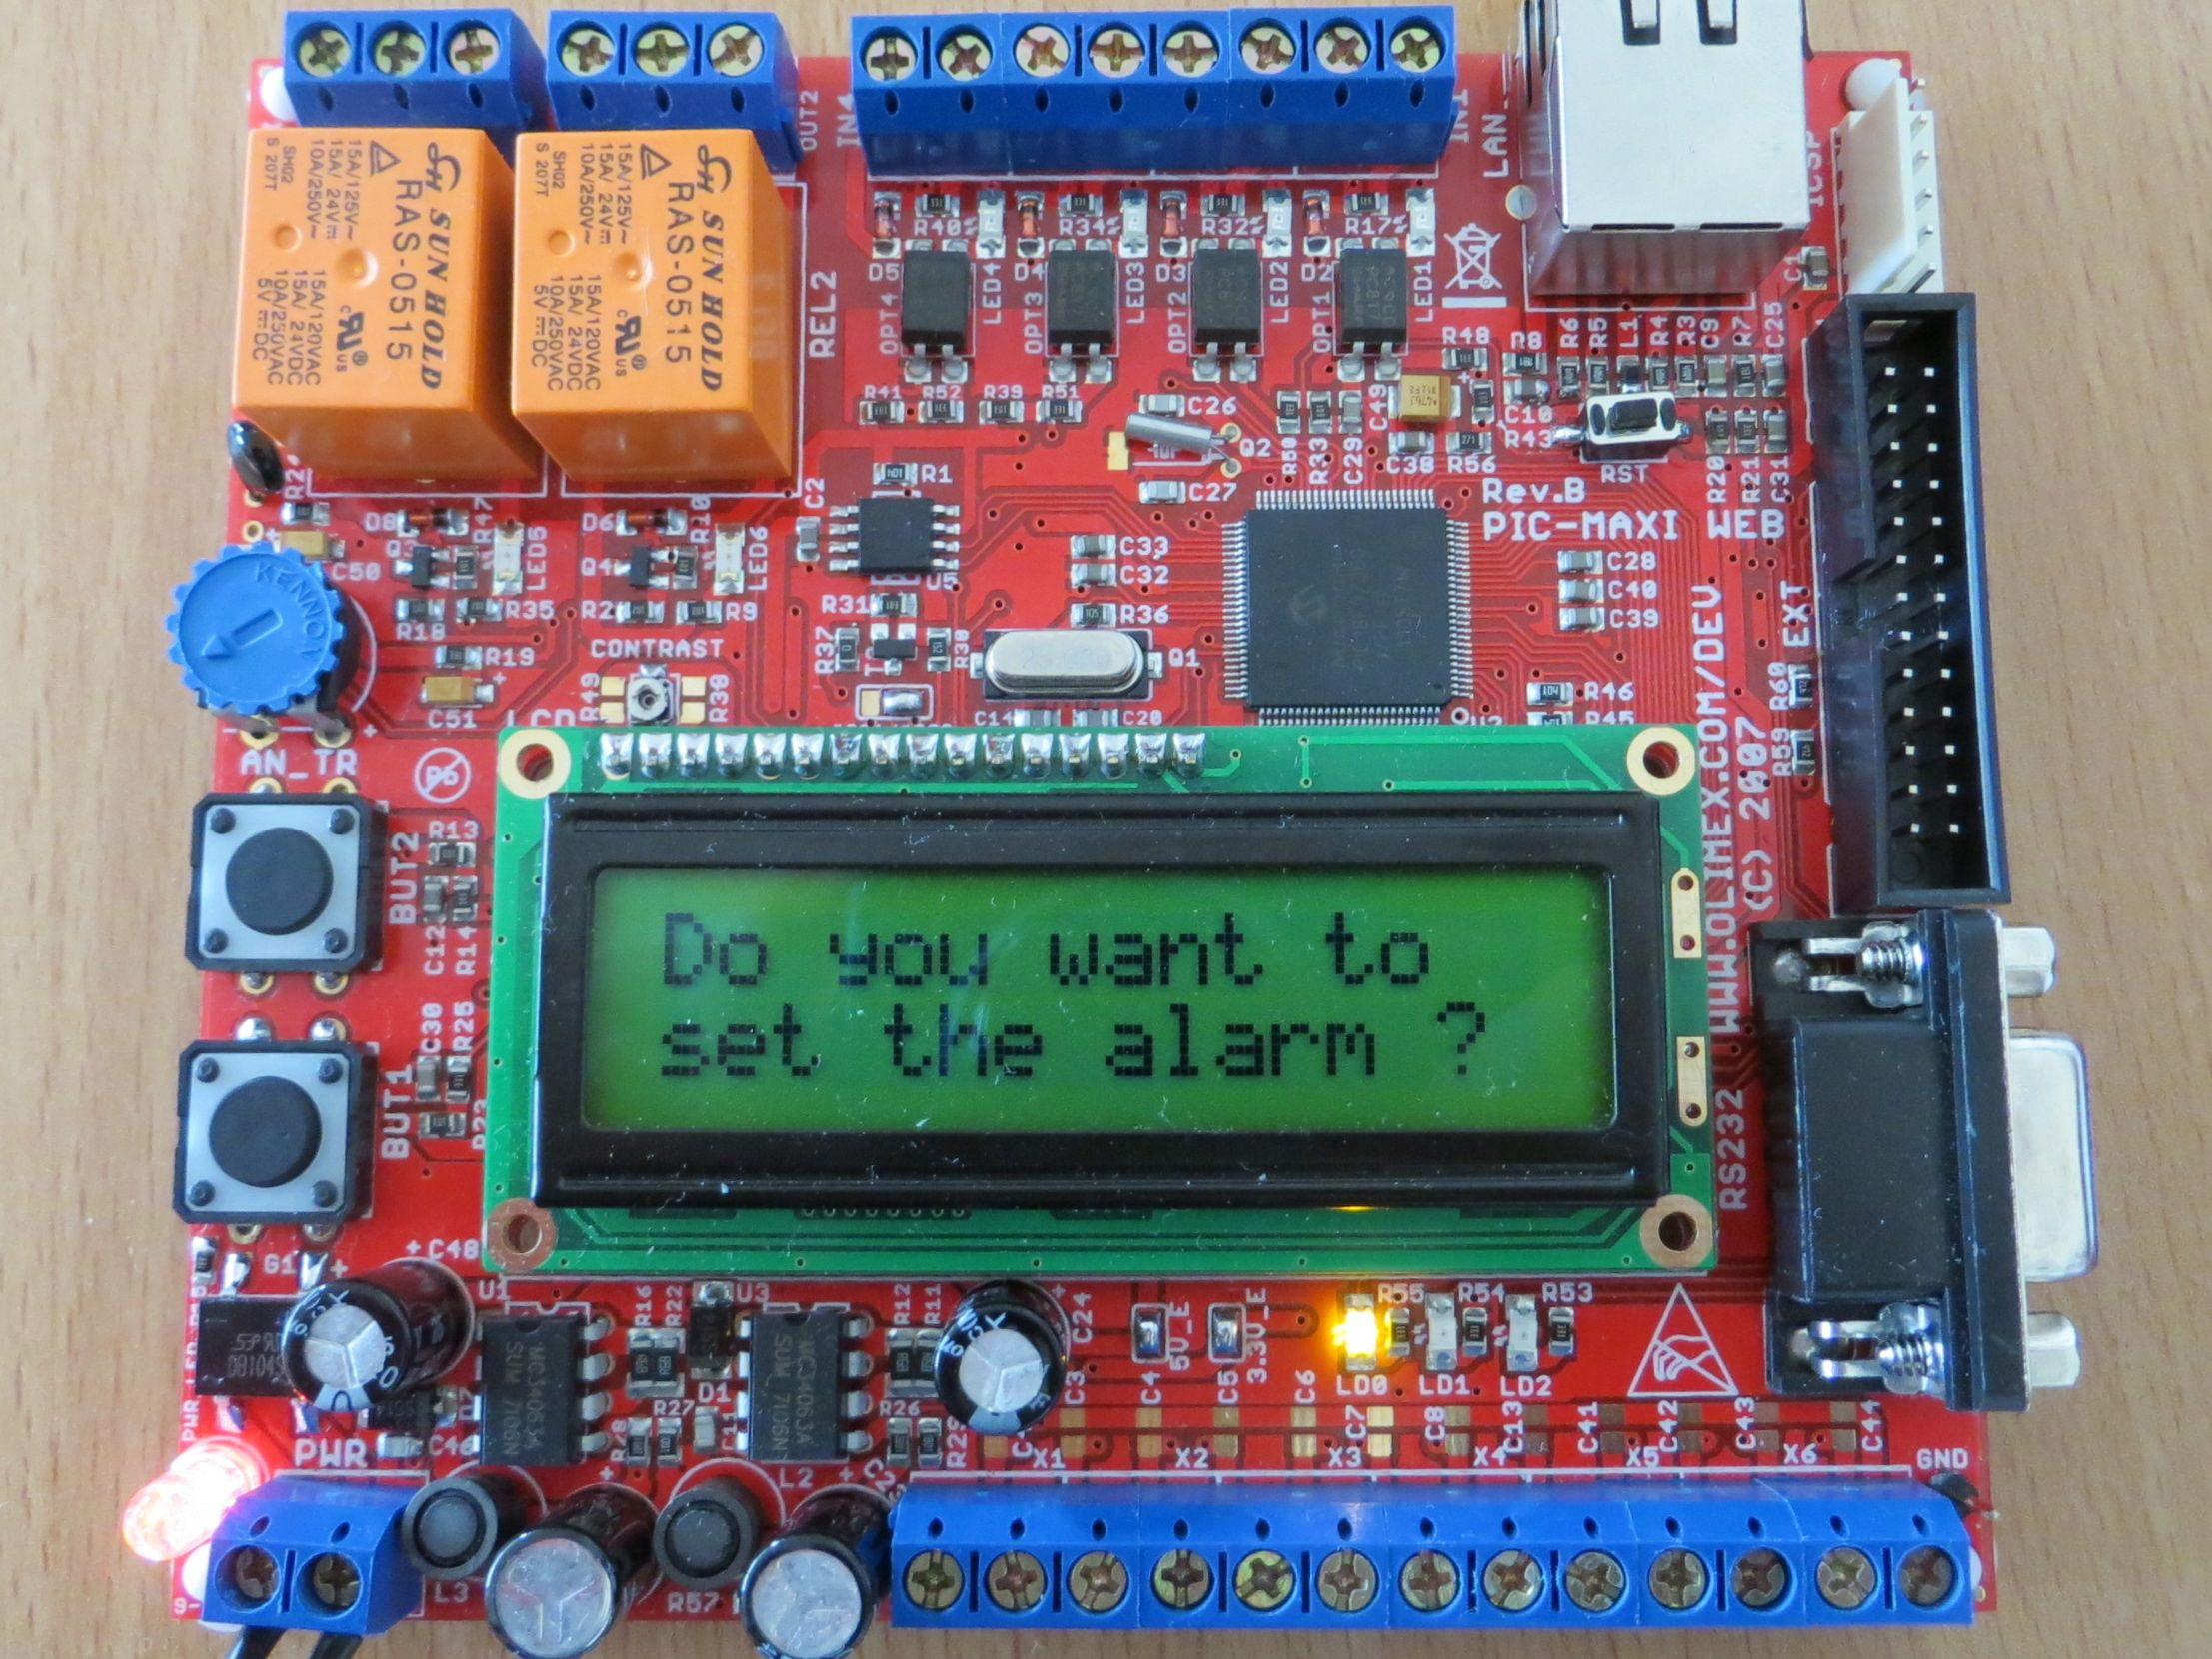
\includegraphics[width=\textwidth]{photos/IMG_2151.JPG}
                \caption{Menu}
                \label{fig:questionalarme}
        \end{subfigure}%
        ~ %add desired spacing between images, e. g. ~, \quad, \qquad etc.
          %(or a blank line to force the subfigure onto a new line)
          \begin{subfigure}[b]{0.4\textwidth}
                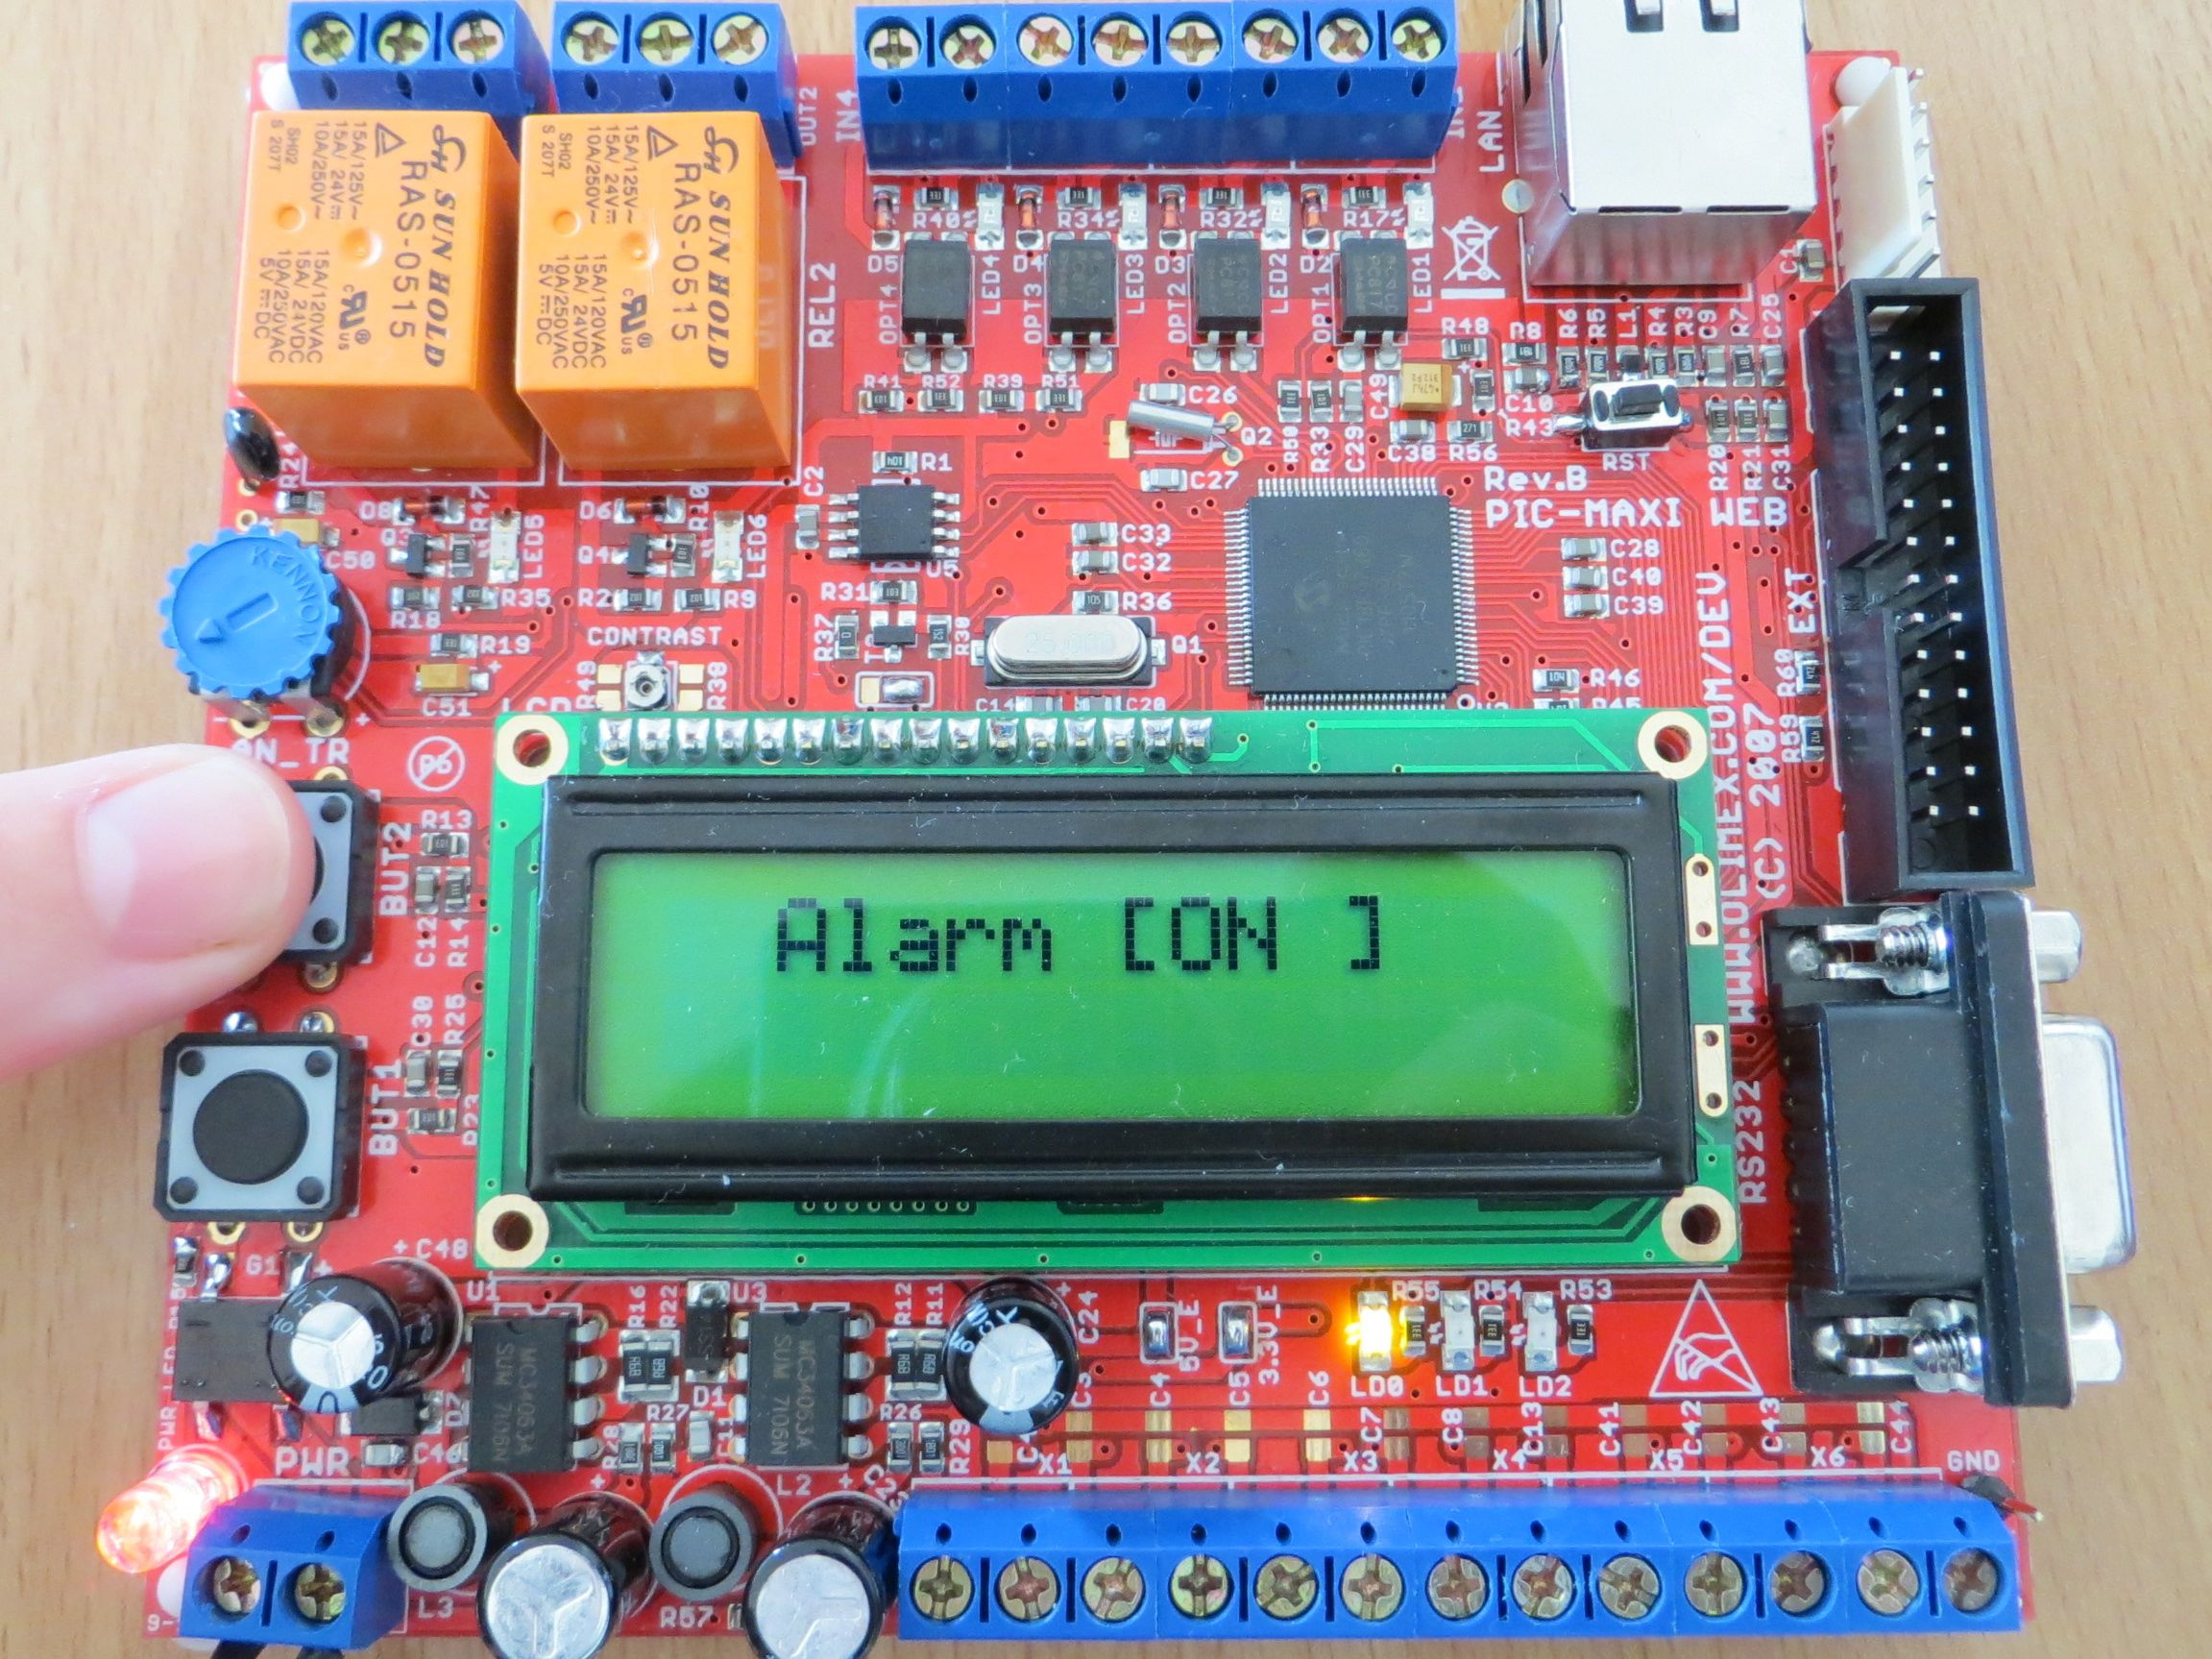
\includegraphics[width=\textwidth]{photos/IMG_2156.JPG}
                \caption{On/off}
                \label{fig:activeralarme}
        \end{subfigure}
        \begin{subfigure}[b]{0.4\textwidth}
                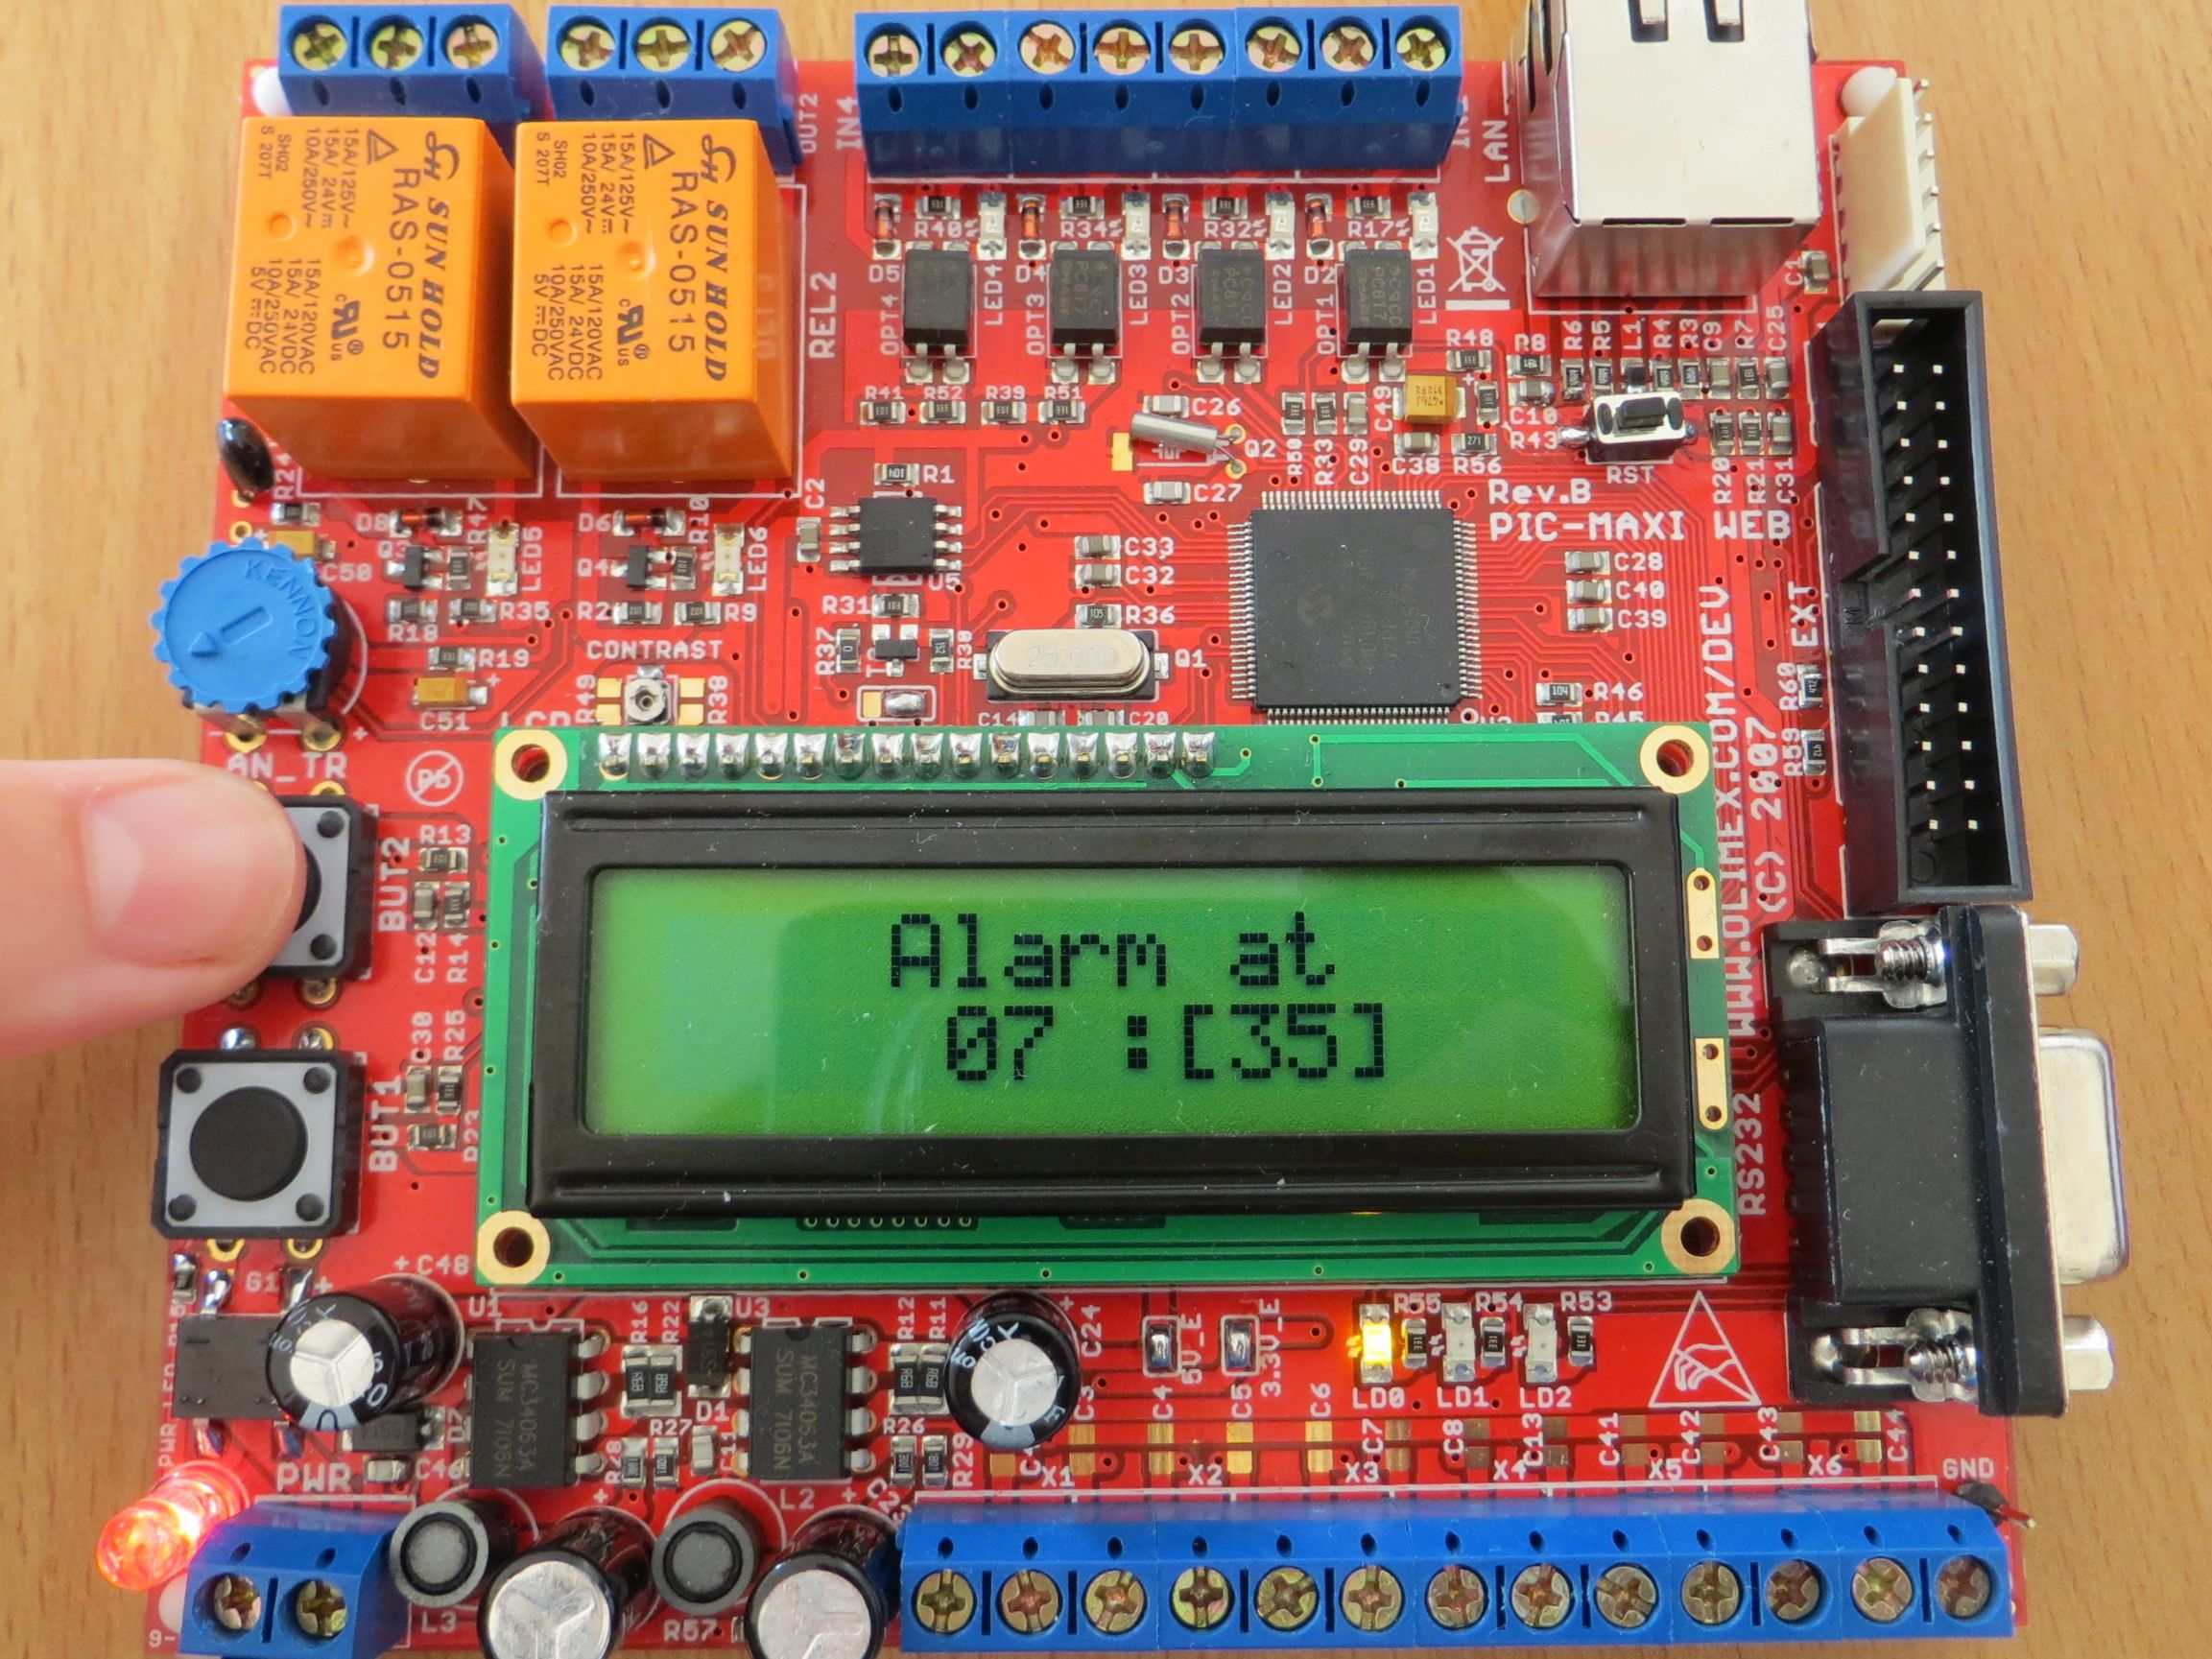
\includegraphics[width=\textwidth]{photos/IMG_2157.JPG}
                \caption{Modification de l'heure}
                \label{fig:modificationalarme}
        \end{subfigure}
        \caption{Modification de l'heure de l'alarme}\label{fig:changeralarme}
\end{figure}

\paragraph{Menu du l'alarme} Si vous désirez revenir à l'affichage de l'heure (Figure~\ref{fig:réveil}), poussez le bouton NEXT; pour régler l'alarme, poussez le bouton SELECT (Figure~\ref{fig:activeralarme}). En appuyant sur ADD, vous pouvez activer ou désactiver l'alarme. L'écran vous indique l'état actuel par ON ou OFF. Le bouton NEXT vous fait accéder à l'heure de l'alarme (Figure~\ref{fig:modificationalarme}), dont vous pouvez changer la valeur en poussant sur ADD. NEXT vous permet de passer aux minutes, que vous pouvez également modifier avec le bouton ADD. Il n'est pas possible de modifier les secondes de l'alarme étant donné que c'est une fonctionnalité que notre équipe technique a jugée inutile. Enfin, le bouton NEXT vous fait quitter le menu et vous amène à l'affichage de l'heure (Figure~\ref{fig:réveil}).

\paragraph{L'affichage}
Le réveil affiche l'heure sous le format hh~:~mm~:~ss sur la première ligne de l'écran. La seconde ligne indique si l'alarme est mise (Figure~\ref{fig:alarmeon}) ou non (Figure~\ref{fig:alarmeoff}) et à quelle heure elle est réglée. Pour accéder au menu (Figure~\ref{fig:questionhorloge}), il suffit d'appuyer sur le bouton MENU et de le parcourir avec les boutons NEXT et SELECT. La LED jaune clignote en continu avec une période de 1 seconde. De cette façon, à n'importe quel endroit du menu, on peut visualiser les secondes qui passent.

\begin{figure}[!h]
        \centering
        \begin{subfigure}[b]{0.5\textwidth}
                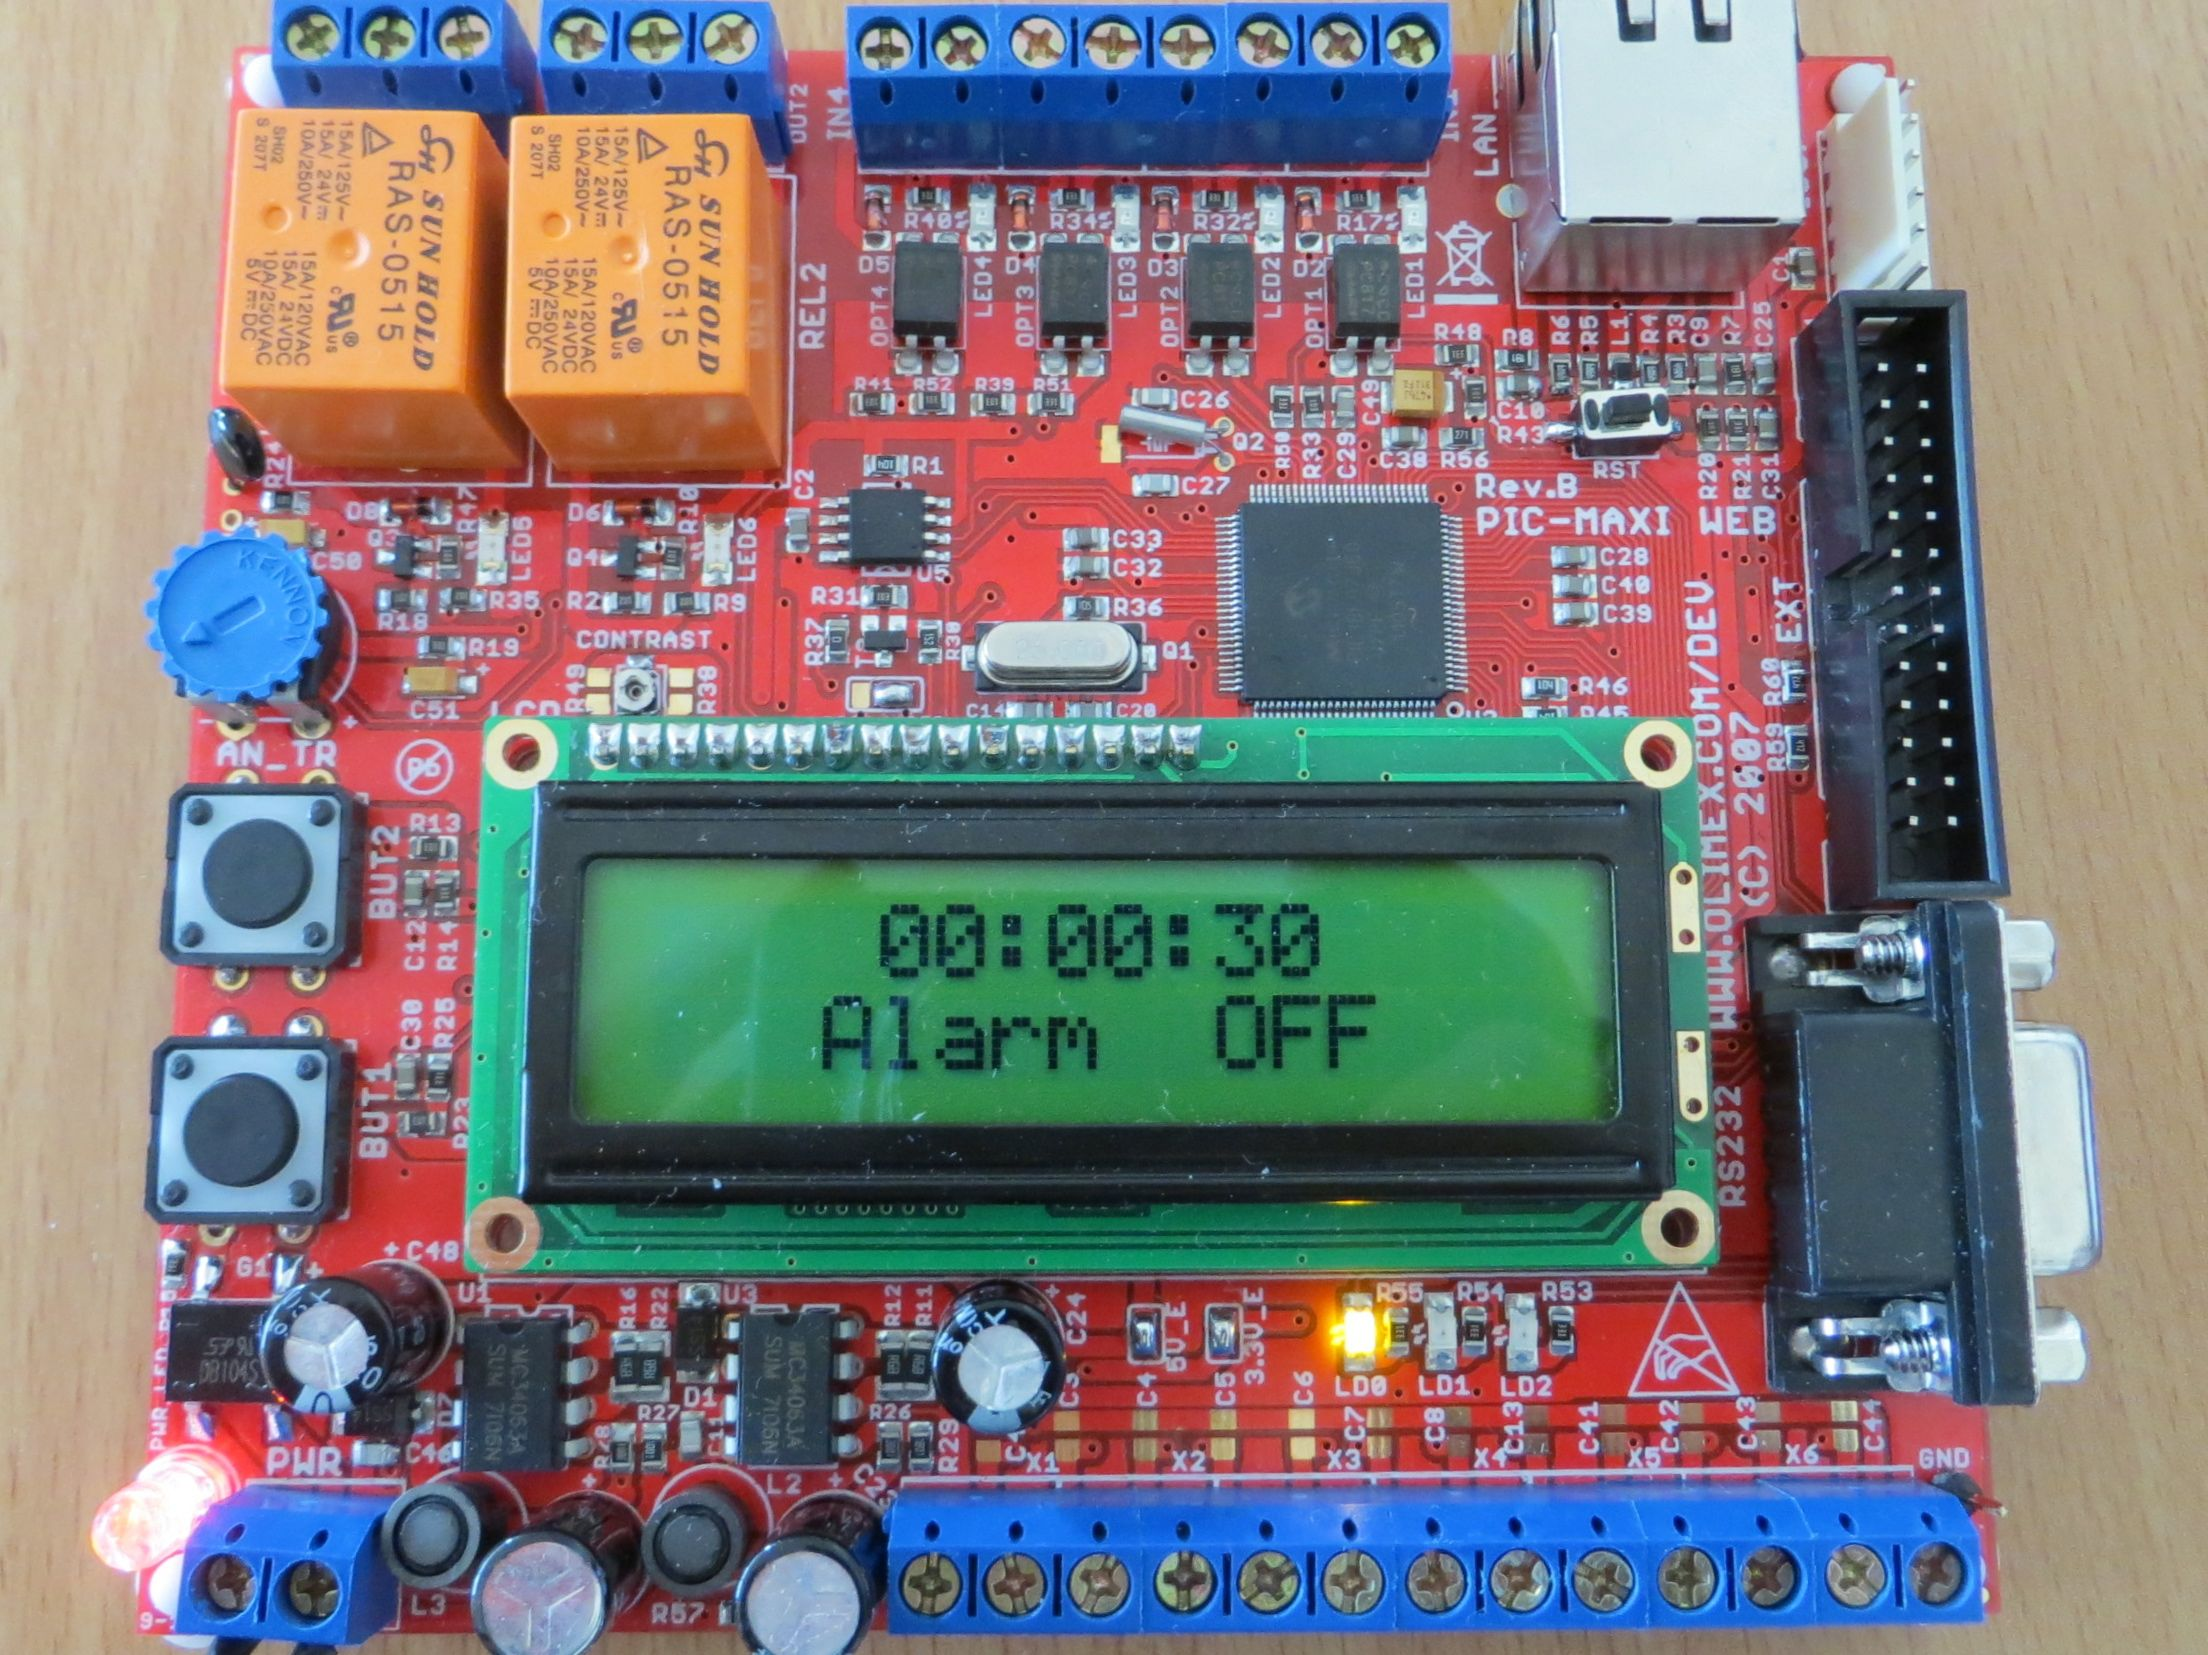
\includegraphics[width=\textwidth]{photos/IMG_2152.JPG}
                \caption{Affichage avec alarme OFF}
                \label{fig:alarmeoff}
        \end{subfigure}%
        ~ %add desired spacing between images, e. g. ~, \quad, \qquad etc.
          %(or a blank line to force the subfigure onto a new line)
        \begin{subfigure}[b]{0.5\textwidth}
                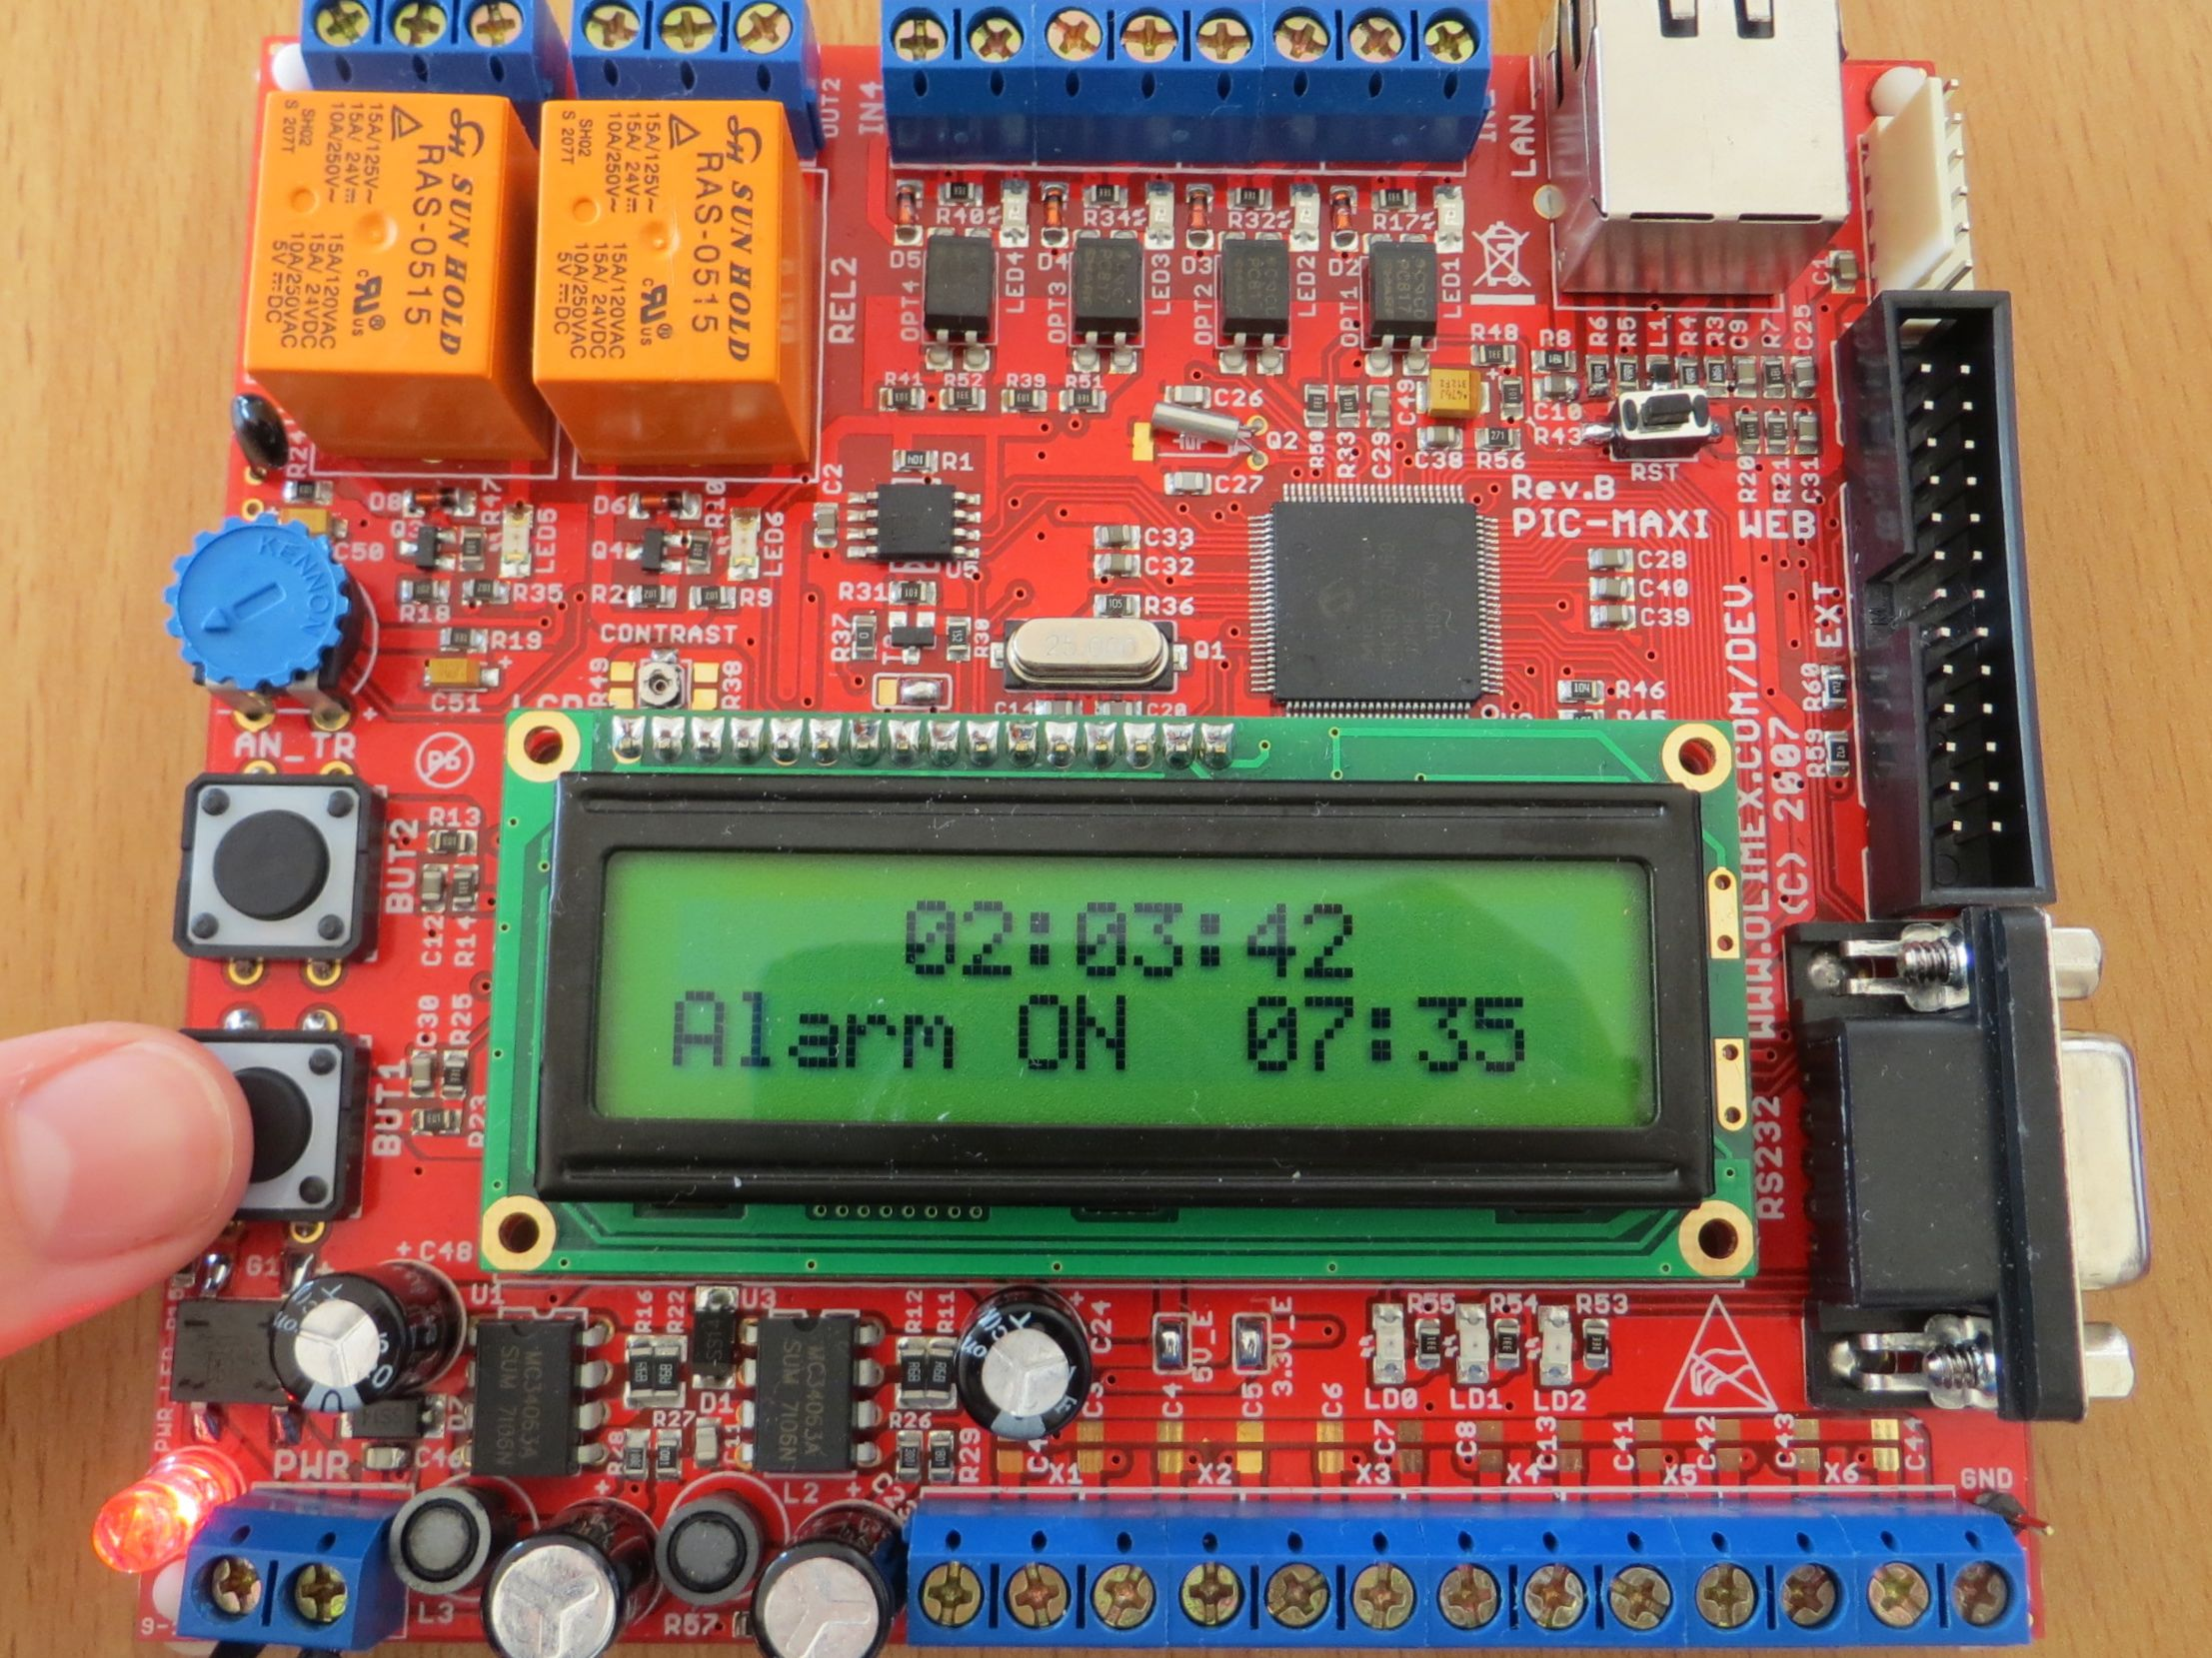
\includegraphics[width=\textwidth]{photos/IMG_2158.JPG}
                \caption{Affichage avec alarme ON}
                \label{fig:alarmeon}
        \end{subfigure}
        \caption{Affichage principal}
        \label{fig:réveil}
\end{figure}

\begin{figure}[!h]
        \centering
        \begin{subfigure}[b]{0.5\textwidth}
                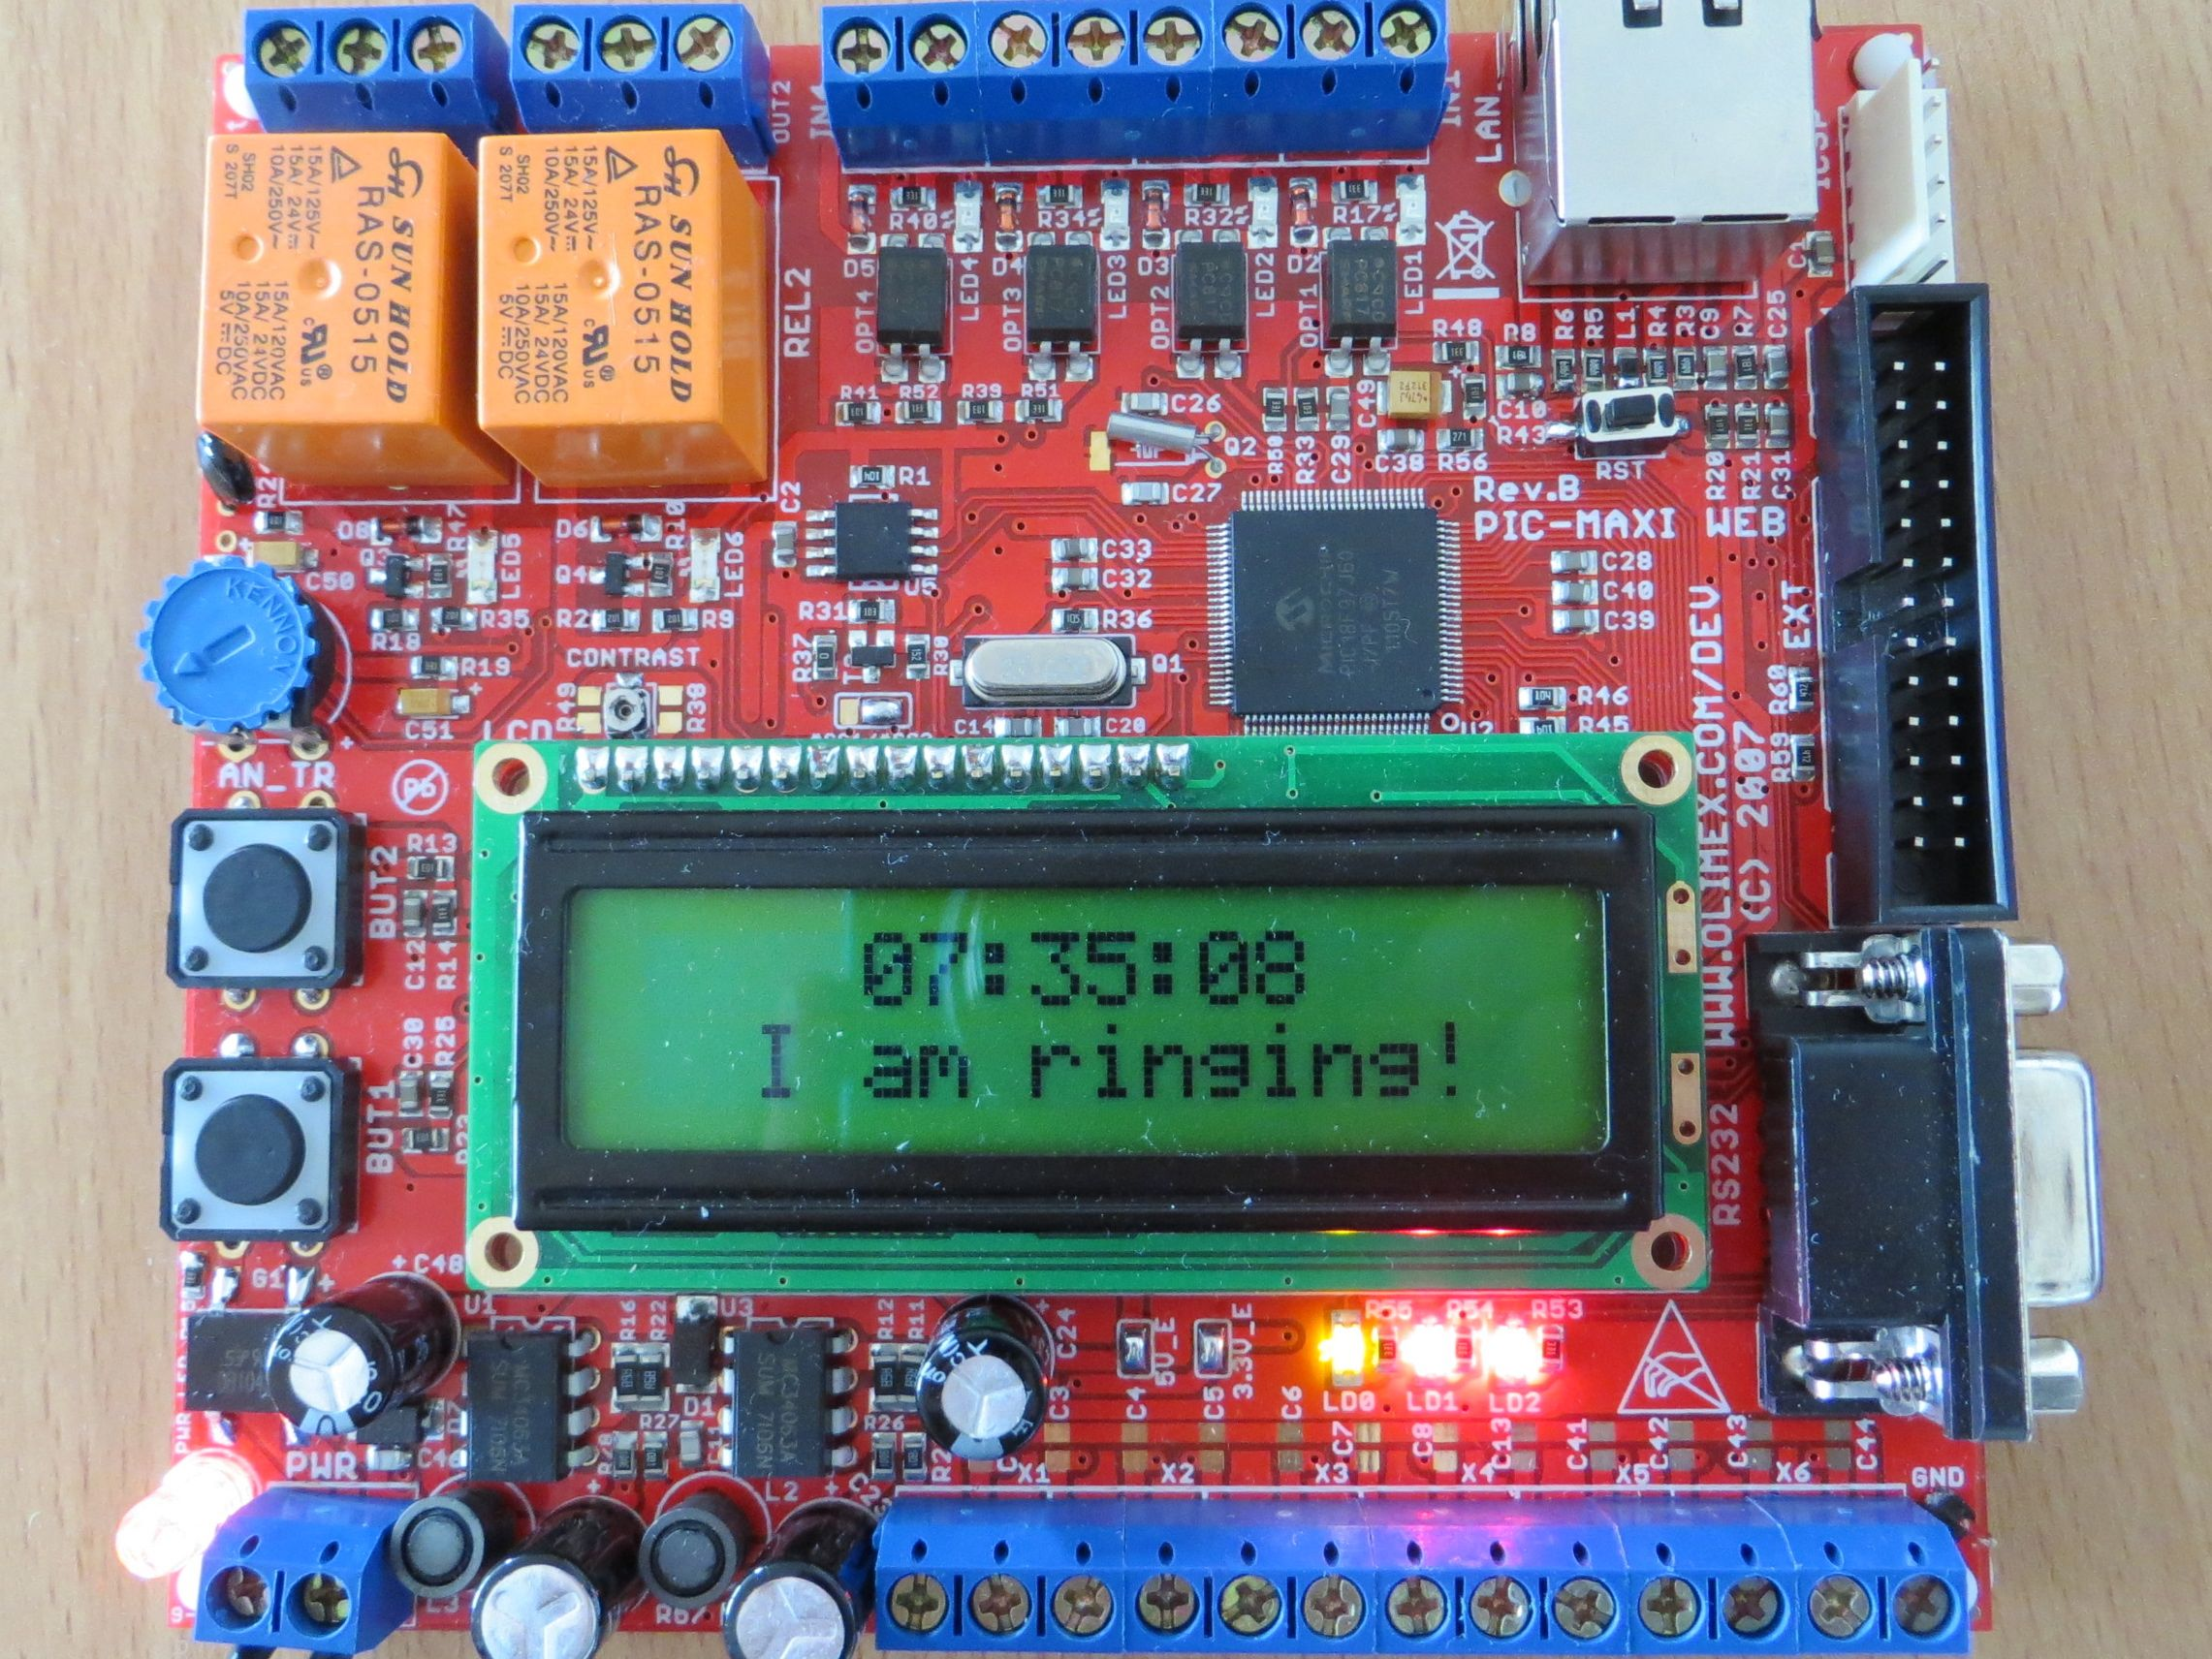
\includegraphics[width=\textwidth]{photos/IMG_2160.JPG}
                \caption{Sonnerie de l'alarme}
                \label{fig:sonneriealarme}
        \end{subfigure}%
        ~ %add desired spacing between images, e. g. ~, \quad, \qquad etc.
          %(or a blank line to force the subfigure onto a new line)
        \begin{subfigure}[b]{0.5\textwidth}
                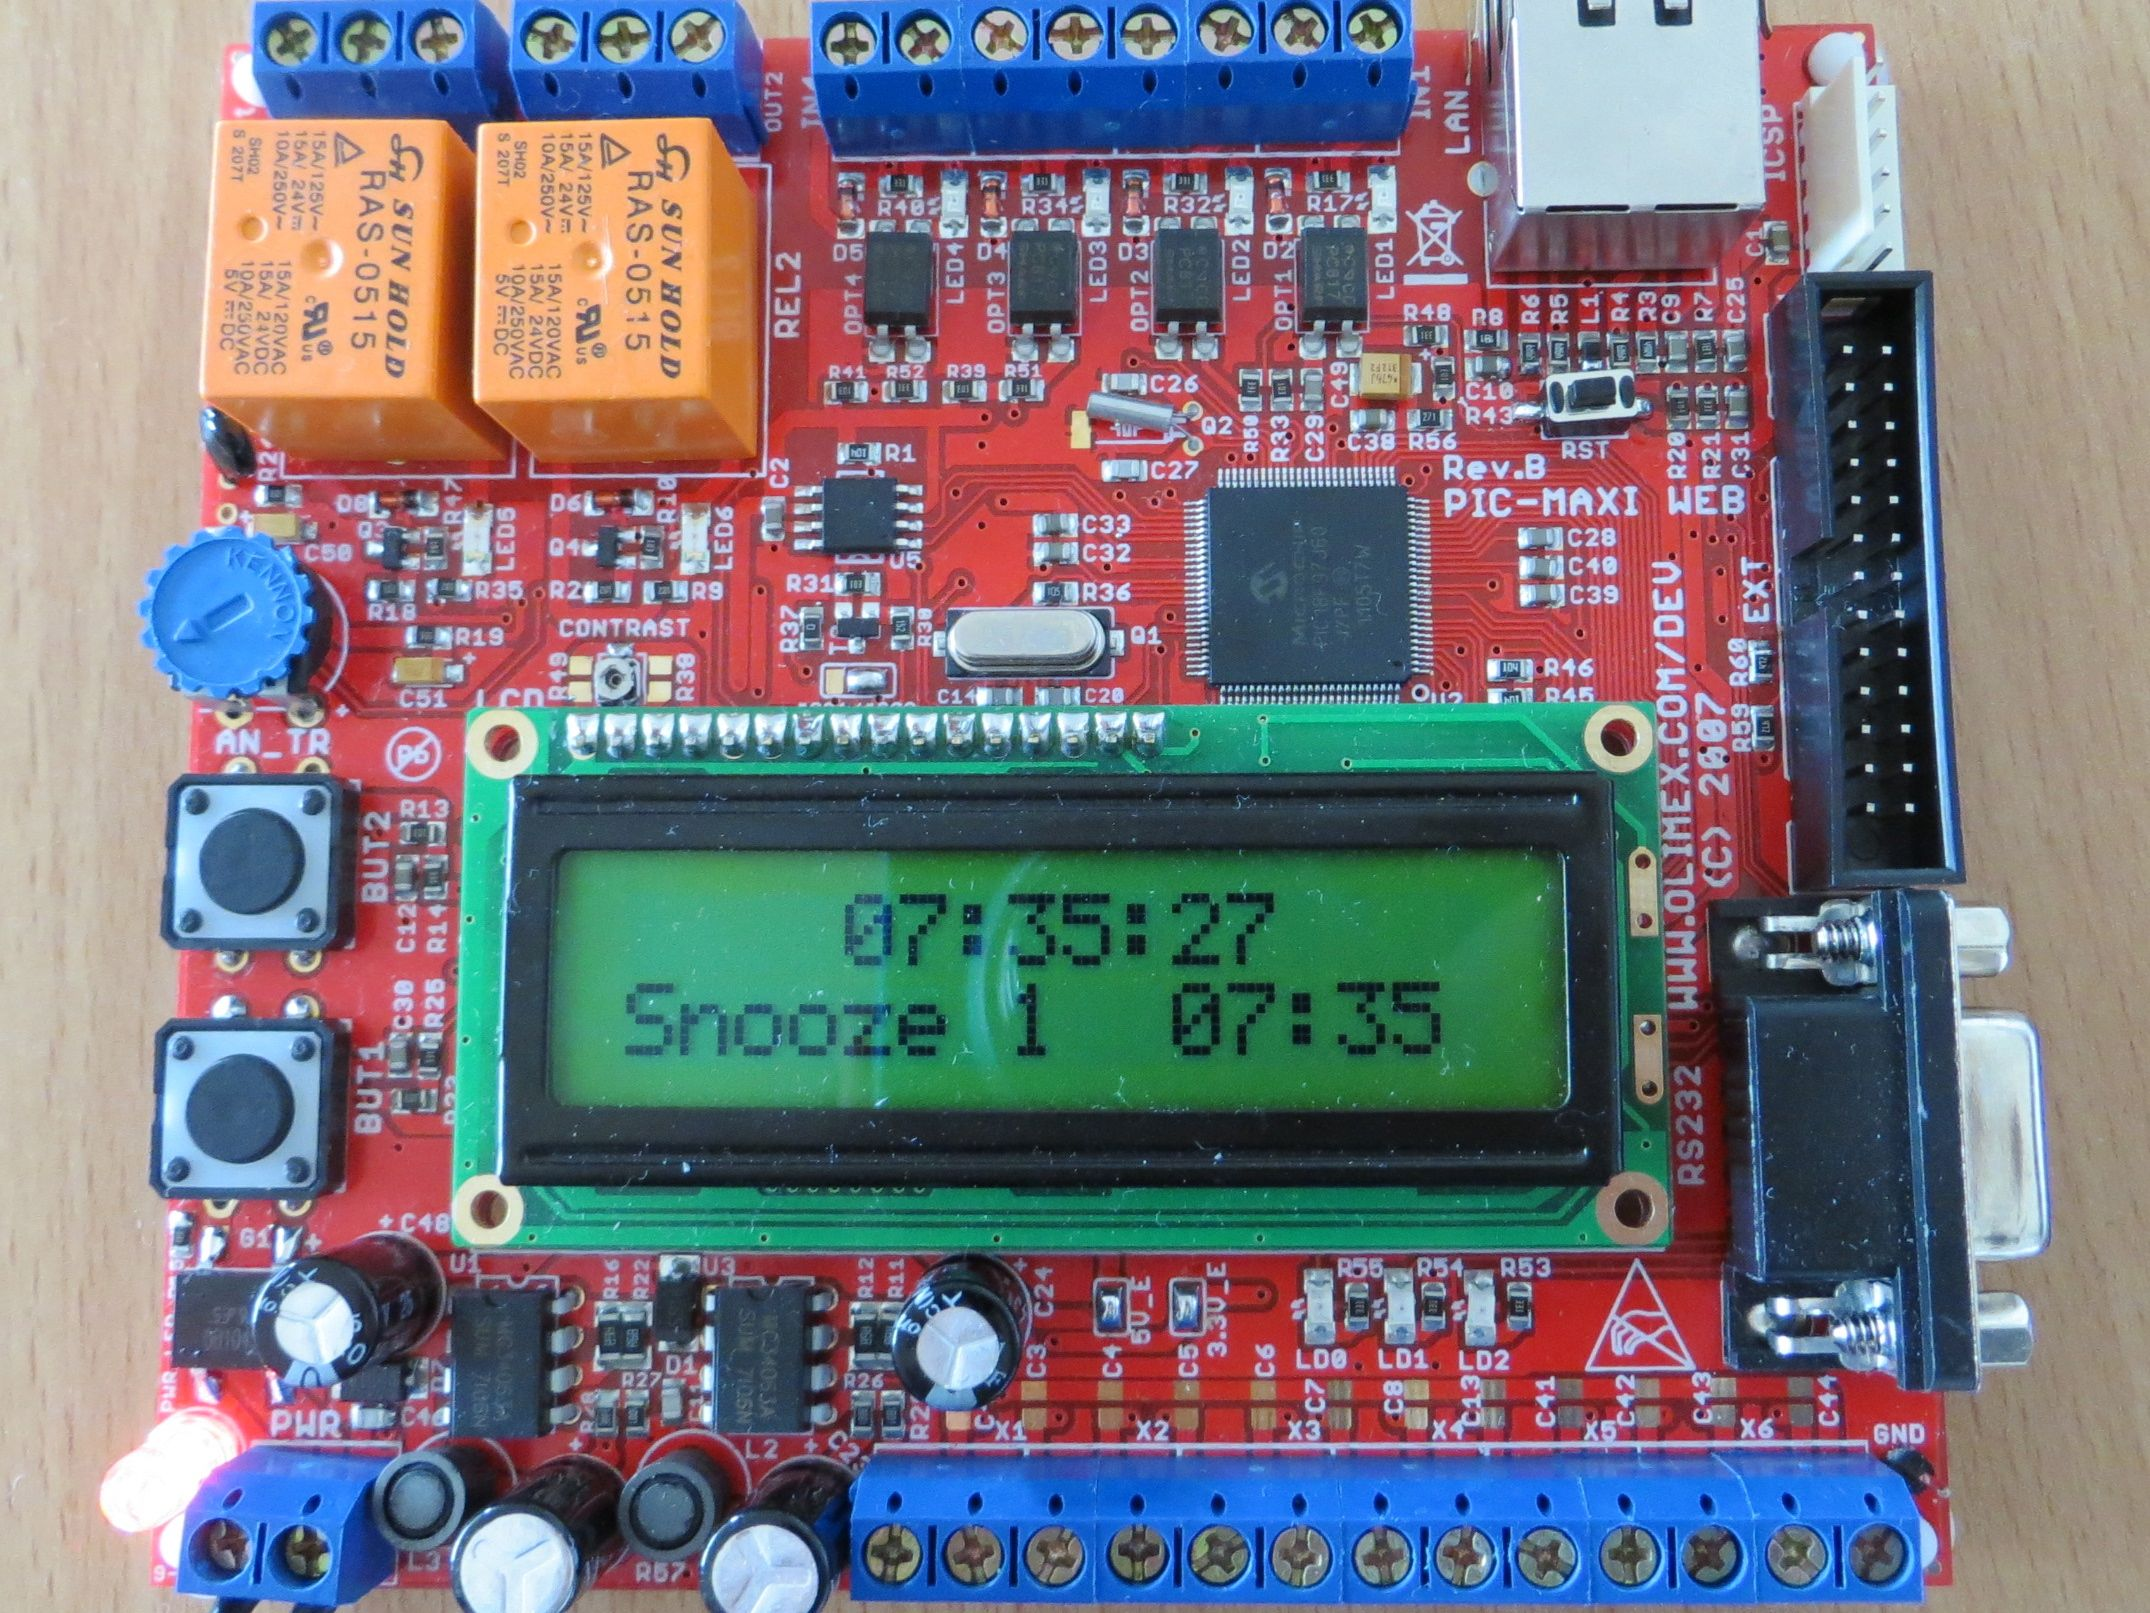
\includegraphics[width=\textwidth]{photos/IMG_2162.JPG}
                \caption{Snooze}
                \label{fig:snoozealarme}
        \end{subfigure}
        \caption{Gestion de la sonnerie de l'alarme}
        \label{fig:sonneriealarme}
\end{figure}

\subsection{Le réveil}
Lorsque le réveil sonne, les deux LED rouges clignotent avec une période de 1 seconde (Figure~\ref{fig:sonneriealarme}). La sonnerie dure 30 secondes, délai après lequel le réveil s'éteint automatiquement. Il reste toutefois activé pour une prochaine utilisation le lendemain.

Lors de l'alarme, il y a deux options possibles~:
\begin{description}
\item[stop] Soit vous souhaitez l'éteindre; il suffit alors d'appuyer sur STOP. Le réveil sonnera à nouveau dans 24 heures.
\item[snooze] Soit vous désirez reporter le réveil de 5 minutes; appuyez alors sur SNOOZE. L'écran vous affiche maintenant l'heure en cours, le nombre de snoozes effectués et l'heure de réveil d'origine (Figure~\ref{fig:snoozealarme}). Pendant le mode snooze, ou à chaque fois que le réveil sonne à nouveau, vous pouvez reporter le réveil de 5 minutes supplémentaires, jusqu'à un maximum de 60 minutes au total. Vous pouvez aussi à tout moment appuyer sur STOP, ce qui aura pour effet d'arrêter le réveil, de revenir à l'affichage normal de l'heure et de remettre l'alarme à l'heure d'origine pour une nouvelle utilisation le lendemain (Figure~\ref{fig:alarmeon}).
\end{description}

Il n'est pas possible d'accéder au menu tant que le réveil n'a pas été éteint. De même, tant que vous êtes dans le menu, le réveil ne sonne pas, pour ne pas interférer avec d'éventuels changements en cours.

\section{Documentation pour l'installateur}
% Les instructions décrivant comment compiler, installer sur le PIC et tester votre programme (documentation pour l'installateur)
Le dossier comprend deux programmes~:
\begin{itemize}
\item \texttt{reveil.c}, le réveil % #### CHANGER LE NOM ####
\item \texttt{findfreq.c}, pour déterminer la fréquence du PIC (vous verrez s'afficher le nombre d'overflows du timer0 après 10 minutes, voir section~\ref{subsec:freq} pour plus de détails)
\end{itemize}
Les instructions suivantes décrivent les étapes à suivre pour installer le réveil sur le PIC. La procédure est la même pour le second programme, il faut juste changer le nom.

\subsection{Compilation}
Pour compiler \texttt{reveil.c}, allez dans le dossier \texttt{PIChorloge/programme/} et tapez la commande \texttt{make reveil} dans le terminal.

\subsection{Installation}
Commencez par brancher le câble d'alimentation du PIC au routeur et mettez-le sous tension (220V AC). Branchez le PIC au port 3 du routeur à l'aide d'un des câbles ethernet; branchez ensuite votre ordinateur au port 2 du routeur avec l'autre câble ethernet. La LED du port 2 du routeur doit s'allumer.

Dans le terminal, tapez les commandes suivantes pour vous connecter au routeur et transférer le fichier \texttt{reveil.hex} au PIC~:
\begin{verbatim}
    my_computer $ tftp 192.168.97.60       // press 'enter'
    my_computer $ tftp> put alarm.hex      // wait!
\end{verbatim}
Avant d'appuyer sur ``enter'' pour le seconde commande, resettez le PIC (petit bouton ``reset'' derrière le port ethernet) et attendez que le LED du port 3 du routeur s'allume. Vous avez à présent 3 secondes pour effectuer le transfert.\\
Pour quitter le client tftp, tapez
\begin{verbatim}
    my_computer $ tftp> quit               // press 'enter'
\end{verbatim}
Le programme se lance automatiquement sur le PIC. Pour le faire redémarrer, appuyez sur le bouton ``reset''.


\section{Documentation pour le programmeur}
% Tout ce qui est nécessaire à un programmeur qui devrait adapter votre programme (documentation pour le programmeur), c'est-à dire, par exemple:
	% Quelle est la fonction du programme (spécification)
    % Quels sont les choix structurels du programme (p. ex. il fonctionne par interruptions et pourquoi)
    % Quelle méthode avez-vous choisie pour mesurer des délais au moyen des timers du PIC et pourquoi
    % Quels sont les autres décisions d'implémentation que vous avez prises et pourquoi vous avez fait ces choix là plutôt que d'autres (même si la raison est que c'est la première idée qui vous est passée par la tête!)
    % Quels sont les détails techniques du PIC qu'il faut avoir en tête pour comprendre le programme
    
    \subsection{Spécifications}
    Le réveil satisfait aux fonctionnalités suivantes~:
    \begin{itemize}
    \item Il affiche l'heure et la met à jour au moins une fois par seconde. Une LED jaune clignote toutes les secondes.
    \item Il contient un réveil qui, activé, ``sonne'' pendant 30 secondes. La sonnerie est remplacée par le clignotment de LED rouges toutes les secondes.
    \item Il est possible de régler l'heure sans interrompre l'horloge.
    \item Il est possible de régler et d'activer/désactiver l'alarme.
    \item Il est possible de postposer l'alarme de 5 minutes pendant une heure.
    \end{itemize}
    
    \subsection{Fréquence du PIC}
    \label{subsec:freq}
    
    Pour déterminer l'heure, nous avons du nous baser sur le timer0 de notre PIC. Ce timer est un registre qui est incrémenté automatiquement à chaque coup d'horloge, et qui, lors d'un débordement (overflow), génère une interruption. Nous avons alors effectué quelques tests nous permettant de mesurer à quelle fréquence ce registre est incrémenté, sur base de quoi nous avons pu ensuite nous baser pour concevoir notre réveil-matin. Nous allons vous présenter ici notre stratégie.\\
  
 Outre le timer0, le PIC contient un timer1 qui peut être programmé pour déborder après exactement 2 secondes (mais nous n'avons toutefois pas eu l'autorisation de l'utiliser dans le cadre du réveil-matin en lui-même).  Notre stratégie a alors été de mesurer le nombre de fois que le timer0 déborde pendant ce laps de temps. Nous estimerons alors que $$f_{software} = \frac{overflows \cdot 2^{16}}{2}$$ car le registre fait 16 bits et $$f_{hardware} = 4 \cdot f_{software}$$ comme expliqué dans la documentation du PIC.\\
 
 Afin d'avoir une erreur relative la plus petite possible, nous n'avons pas utilisé de prescaler sur le timer0 (option qui permet de diviser la fréquence d'incrémentation du registre par une puissance de 2) et avons effectué notre mesure sur plus de 2 secondes. En effet, si on considère ici f comme étant la fréquence hardware, qu'on appelle $value$ est la valeur qui se trouve dans le timer0 pile au moment de l'overflow du timer1 et $N$ est le temps de notre mesure en secondes, nous pouvons aussi écrire
 \begin{eqnarray*}
 f_{exacte} &=& \frac{4 \cdot (overflows \cdot 2^{16} + value)}{N}\\
f_{mesurée} &=&  \frac{4 \cdot (overflows \cdot 2^{16})}{N}\\
 \text{erreur relative} &=& \frac{|f_{exacte} - f_{mesurée}|}{f_{exacte}}\\
                      &=& \frac{value}{overflows \cdot 2^{16} + value}\\
\end{eqnarray*}
 Notre erreur relative sera donc plus petite lorsque overflows est plus grand. C'est pourquoi utiliser un prescaler sur le timer0 serait contreproductif (cela diminuerait le nombre d'overflows) et augmenter le temps de mesure est intéressant (cela augmentera le nombre d'overflows).\\
 
 Nous avons pris le parti de ne pas mesurer la valeur se trouvant dans le timer0 après l'overflow du timer1 parce que cette valeur est négligeable. L'erreur relative maximale en ne la mesurant pas est en effet $\leq \frac{1}{overflows + 1}$. De plus, on ne trouverait de toute façon pas précisément la valeur qui se
 trouvait dans le timer0 pile au moment de l'overflow.\\
 
Nous avons donc créé un programme \texttt{findfreq.c} qui compte et affiche le nombre d'overflows sur sur un laps de temps de 10 minutes. Nous avons effectué 3 mesures avons trouvé qu'en moyenne
  \begin{eqnarray*}
 \text{le nombre d'overflows/s} &=& 95,366\\
f_{software}  &=& 95,366 \cdot 2^{16} = 6249906,176\\
f_{hardware} &=& 6249906,176 \cdot 4 = \unit{24999624}{\hertz}
 \end{eqnarray*}
 ce qui représente un écart de seulement 0.0015\% par rapport à la fréquence de \unit{25}{\mega\hertz} annoncée dans la documentation du PIC.
 
    \subsection{Choix d'implémentation}
    
    \subsubsection{Mesure du temps}
    %Comme expliqué dans la section~\ref{subsec:freq}, nous avons trouvé qu'en moyenne 1 seconde correspond à $95.366$ overlflows du timer0. C'est cette donnée qui nous a permis dans notre programme de calculer l'heure. 
    
    Plusieurs choix d'implémentation s'offraient à nous.\\
    
    Tout d'abord, il a fallu choisir si nous voulions nous servir d'interruptions ou faire de l'attente active, c'est-à-dire examiner régulièrement la valeur du timer dans une boucle jusqu'à ce qu'il atteigne la valeur souhaitée. Nous avons décidé de nous servir des interruptions parce qu'elles prennent le dessus sur le restant du programme. Comme le calcul du temps se base sur le nombre d'overflows, l'incrémentation de ce compteur doit être prioritaire par rapport au reste.\\
    
    Un deuxième choix, indépendant du premier, est de laisser le temporisateur tourner librement ou non. Ce qu'on entend par ne pas laisser tourner le compteur librement est changer la valeur dans le timer à un moment donné. Par exemple, on pourrait calculer le nombre d'incrémentations qui correspondent à 1 seconde et se dire qu'on va changer la valeur dans le timer0 à $2^{16}$ moins cette valeur afin qu'il déborde après une seconde. Cette technique a un inconvénient majeur : il y a un délai entre le débordement du compteur et le moment où on le réinitialise : il faut donc soustraire de la valeur calculée précédemment la valeur du compteur au moment où on le réinitialise. Cette valeur est difficile à calculer de façon précise et pourrait en plus à priori ne pas être constante. Nous avons donc rejeté cette solution et avons décidé de laisser tourner le compteur librement.\\
    
    Un autre choix à effectuer a été d'utiliser le prescaler ou non. Nous avons décidé de ne pas l'utiliser tout simplement parce que cela diminuerait la fréquence d'incrémentation du timer0 et augmenterait donc l'incertitude sur le temps écoulé. Au contraire, il aurait plutôt été intéressant de l'augmenter. Mais cela n'est pas possible et on prendrait le risque que des interruptions ne soient pas traitées parce qu'elles arrivent en même temps qu'une autre. Notons que, sans prescaler, nous ne pensons pas que ce type d'événement arrive souvent vu la fréquence très proche de \unit{25}{MHz} que nous avons trouvée. \\
    
    Il nous a ensuite fallu établir une vraie stratégie permettant de calculer l'heure sur base des interruptions du timer0 s'incrémentant normalement. Une première idée que nous avons eue était d'avoir des variables heure, minute et seconde et un compteur d'overflows "qui n'ont pas encore été traités". Supposons que nous avions trouvé qu'il fallait 95,5 overflows pour avoir 1 seconde. Nous aurions alors défini qu'à chaque fois que overflows dépasse un multiple de $95$, on incrémentait nos secondes de 1 (avec une bonne gestion de valeurs maximales des variables et des reports entre elles évidemment) et nous aurions ensuite corrigé l'erreur commise en disant qu'une fois que overflows $= 2\cdot 95$, nous remettions overflows à $-1$ afin de corriger l'erreur commise en disant que la fréquence valait 95. Cette technique n'est cependant pas du tout applicable dans notre cas car nous avons trouvé $95,336$ overflows ce qui fait que pour garder une telle précision, il faudra attendre $500$ secondes et mettre overflows à $-168$, ce qui correspond à plus d'une seconde à retirer. Cela veut dire que soudainement on aurait un recul d'une seconde qui se verrait clairement sur le LCD et ce n'est pas ce que nous désirons.\\
    
    Ce que nous avons finalement fait pour garder notre précision est de garder un compteur du nombre d'overflows depuis le lancement du programme. Nous pouvons ensuite convertir ce compteur en un délai heure, minute, seconde sur base de simples calculs basés sur le fait que $1$ seconde correspond à $95,336$ overflows. Il suffit alors de modifier ces variables lorsque nos calculs aboutissent à des valeurs différentes. La modification de l'heure par l'utilisateur modifiera donc directement cette unique valeur aussi. Il faudrait juste ajouter à overflows le nombre d'overflows adéquat.\\

    % Notre réveil se base sur le timer0 pour mesurer le temps qui passe.
 %Connaissant la fréquence de celui-ci, il compte le nombre d'overflows et
 %vérifie si une seconde est passée pour mettre à jour l'heure de l'horloge.
    \subsubsection{\'Etats du réveil}
    Le réveil peut se trouver dans 11 états différents. Ils sont définis en début de programme au moyen de \texttt{\#define}. Ils permettent de structurer le code de manière claire et de gérer chaque événement dans son contexte.
    \begin{itemize}
    \item[\texttt{TIME\_MENU 1}:] Permet d'accéder au menu de l'horloge.
	\item[\texttt{SET\_HOUR 2}:] Permet de changer l'heure de l'horloge.
	\item[\texttt{SET\_MINUTE 3}:] Permet de changer les minutes de l'horloge.
	\item[\texttt{SET\_SECOND 4}:] Permet de changer les secondes de l'horloge.
	\item[\texttt{ALARM\_MENU 5}:] Permet d'accéder au menu de l'alarme.
	\item[\texttt{SET\_ALARM 6}:] Permet d'activer/désactiver l'alarme.
	\item[\texttt{SET\_A\_HOUR 7}:] Permet de changer l'heure du réveil.
	\item[\texttt{SET\_A\_MIN 8}:] Permet de changer les minutes du réveil.
	\item[\texttt{DISPLAY 9}:] Affichage normal.
	\item[\texttt{ALARM 10}:] Le réveil sonne.
	\item[\texttt{SNOOZE 11}:] Le réveil a été reporté.\\
    \end{itemize}
    
    A chacun de ces états correspond 
    \begin{itemize}
    \item un affichage sur le LCD repris dans la méthode \texttt{refresh\_lcd()} et
    \item une modification à appliquer si on appuie sur l'un des deux boutons repris dans la méthode \texttt{button()}.
    \end{itemize} 
    \subsubsection{\texttt{main()}}
    Après l'initialisation des différents registres nécessaires à son fonctionnement, le programme tourne en boucle pour vérifier
    \begin{itemize}
    \item si l'heure a changé et quelles LED il faut allumer ou éteindre (\texttt{time()})
    \item s'il faut mettre à jour l'affichage (\texttt{refresh\_lcd()})
    \item s'il faut lancer ou arrêter l'alarme (\texttt{alarm()})
    \item sil'utilisateur a appuyé sur un bouton (\texttt{button()}).
    \end{itemize}
    
    \subsubsection{Interruptions}
    % Il y a deux routines d'interruptions à des niveaux de priorités différents :
 %   - le niveau 1 génère une interruption dès que le timer0 overflow et ne
 %    fait que compter le nombre d'overflows qui se sont produits;
 % - le niveau 2 génère une interruption lorsqu'on appuie sur un bouton et
%      modifie le flag du bouton correspondant.
 
 %La fonction main vérifie en boucle
  %  - si le temps mesuré a changé, càd s'il y a eu assez d'overflows pour
  %    ajouter une seconde;
  %  - s'il faut changer l'affichage à l'écran, ce qui arrive lorsque le temps
%      a changé, lorsqu'on a appuyé sur un bouton et lorsque l'alarme se
%      déclenche (càd lorsque l'état du réveil indiqué dans la variable
%      'whereami' a changé);
%    - s'il faut déclencher ou arrêter l'alarme;
%    - s'il faut changer d'état ou la valeur d'une variable suite à
%      l'actionnement d'un bouton.

    \subsection{Détails techniques du PIC}
    
    
\section{Conclusion}
    
\end{document}